\documentclass{article}

\usepackage{cmap} % чтобы работал поиск по PDF

\usepackage{caption}  %-  вставить в krctran перед описанием подписей caption (\renewcommand\@makecaption)
\usepackage{subcaption} % float figures side by side}  -  вставить в krctran перед описанием подписей caption (\renewcommand\@makecaption)
\usepackage{krctran}
%\usepackage[utf8]{inputenc} % закомментировать в krctran.sty: \RequirePackage[cp1251]{inputenc}
\usepackage[pdftex]{graphicx} % закомментировать в krctran.sty
%\usepackage{caption}  %-  вставить в krctran перед описанием подписей caption (\renewcommand\@makecaption)
%\usepackage{subcaption} % float figures side by side}  -  вставить в krctran перед описанием подписей caption (\renewcommand\@makecaption)
\usepackage{textcomp}
\usepackage{xcolor}
\usepackage{algorithm2e}
\usepackage{float}
\usepackage{wrapfig}
%\usepackage[dvips]{graphicx}
\graphicspath{ {./pictures/} }

\begin{document}

\procname{Труды Карельского научного центра РАН\\ \No 0. 2015. С.~1--24}
\udk{УДК 81.32}

\rustitle{Обзор методов и алгоритмов разрешения \newline лексической многозначности: Введение}
\engtitle{Word-sense disambiguation methods and algorithms review: Introduction}

\rusauthor{Т.~В.~Каушинис$^2$,  А.~Н.~Кириллов$^1$,  Н.~И.~Коржицкий$^2$, А.~А.~Крижановский$^1$, А.~В.~Пилинович$^2$, И.~А.~Сихонина$^2$,  А.~М.~Спиркова$^2$, В.~Г.~Старкова$^1$, Т.~В.~Степкина$^2$, С.~С.~Ткач$^2$, Ю.~В.~Чиркова$^1$, А.~Л.~Чухарев$^1$,  Д.~С.~Шорец$^2$,  Д.~Ю.~Янкевич$^2$, Е.~А.~Ярышкина$^2$}
\engauthor{T.~V.~Kaushinis$^2$, A.~N.~Kirillov$^1$, N.~I.~Korzhitsky$^2$, A.~A.~Krizhanovsky$^1$, A.~V.~Pilinovich$^2$, I.~A.~Sikhonina$^2$, A.~M.~Spirkova$^2$, V.~G.~Starkova$^1$, T.~V.~Stepkina$^2$, S.~S.~Tkach$^2$, J.~V.~Chirkova$^1$, A.~L.~Chuharev$^1$, D.~S.~Shorets$^2$, D.~Y.~Yankevich$^2$, E.~A.~Yaryshkina$^2$}


\organization{$^1$Институт прикладных математических исследований Карельского научного центра РАН \\
$^2$Петрозаводский Государственный Университет}


\rusabstract{Разрешение лексической многозначности --- это задача выбора между разными значениями 
слов и словосочетаний в словаре в зависимости от контекста. 
В статье представлен краткий обзор методов и алгоритмов разрешения лексической многозначности. 

Представлены (1) методы, основанные на машинном обучении, 
(2) методы, не использующие никаких размеченных корпусов для различения значений слов, и 
(3) методы, использующие внешние словарные источники информации (машиночитаемые словари, тезаурусы, онтологии). 
Статья распространяется на правах свободной лицензии “CC Attribution”.
}
\engabstract{The word-sense disambiguation  task is the classification task, where the goal is to predict the meaning of words and phrases with the help of surrounding text. The purpose of this short review is to acquaint the reader with the general directions of word sense disambiguation methods and algorithms. The paper consists of three main parts: (1) supervised (machine learning) approaches to word-sense disambiguation, (2) unsupervised approaches based on unlabeled corpora and (3) knowledge-based approaches to word-sense disambiguation, where machine-readable dictionaries, thesauri, ontologies are used. This work is licensed under the CC Attribution license.}

\ruskeywords{алгоритм, метод, разрешение лексической многозначности.}
\engkeywords{algorithm, method, word-sense disambiguation.}

\maketitle

\begin{articletext}
\section{Введение}
В статье представлен обзор методов и алгоритмов разрешения лексической многозначности (word-sense disambiguation или WSD). Верный выбор в словаре одного из значений многозначного слова или фразы в зависимости от контекста является успешным результатом решения WSD-задачи.

Приведем несколько примеров употребления слов <<коса>> и <<косой>>, найденных с помощью Национального корпуса русского языка (http://ruscorpora.ru) по запросу <<коса>>:

\begin{enumerate}
\item Поп сам в первой \textit{\underline{косе}} идет, но прихожане не торопятся, смотрят на солнышко и часа через полтора уже намекают, что обедать пора. {\footnotesize[\textit{М. Е. Салтыков-Щедрин. Мелочи жизни (1886-1887)}]}
\item Но работа даже и после этого идет все вялее и вялее; некоторые и \textit{\underline{косы}} побросали. {\footnotesize[\textit{М. Е. Салтыков-Щедрин. Мелочи жизни (1886-1887)}]}
\item В особенности жестоко было крепостное право относительно дворовых людей: даже волосы крепостных девок эксплуатировали, продавая их \textit{\underline{косы}} парикмахерам. {\footnotesize[\textit{М. Е. Салтыков-Щедрин. Мелочи жизни (1886-1887)}]}
\item Это одинокая скала, соединяющаяся с материком намывной \textit{\underline{косой}} из песка и гальки. {\footnotesize[\textit{В. К. Арсеньев, «По Уссурийскому краю», 1917 г.}]}
\item Первая черепашка подскочила к гвардейцу и воткнула ему в спину сверкающий \textit{\underline{косой}} меч. {\footnotesize[\textit{Виктор Пелевин. S.N.U.F.F, 2011}]}
\end{enumerate}

Первые четыре примера дают три разных значения существительного <<коса>>: ряд косарей, сельскохозяйственное орудие, заплетенные волосы, протяженная речная отмель. Последний пример содержит прилагательное <<косой>>, совпадающее с одной из форм существительного <<коса>>. Все эти значения и часть речи читатель легко определяет по контексту. 

Именно многозначность слов, их неоднозначность и зависимость значений слов от контекста являются причиной возникновения такой задачи и одновременно обуславливают сложность ее решения. Уверенное решение WSD-задачи необходимо во многих приложениях, связанных с автоматической обработкой текста (информационный поиск, машинный перевод и тому подобное) и, на наш взгляд, является предтечей искусственного интеллекта.

Для этой задачи известно большое количество алгоритмов и методов решения, которые можно разделить на \cite{Lukash 2011}, \cite{Navigli 2009}: 

\begin{itemize}
\item WSD-методы с учителем (\textit{supervised}) --- методы, базирующиеся на машинном обучении и работающие на размеченных корпусах текстов; 
\item WSD-методы без учителя (\textit{unsupervised}), не использующие никаких размеченных корпусов для различения значений слов.
\end{itemize}

Другая классификация методов строится на противопоставлении используемых ресурсов \cite{Navigli 2009}:
\begin{itemize}
\item WSD-методы, основанные на знаниях (\textit{knowledge-based}); в этих методах используются внешние словарные источники информации (машиночитаемые словари, тезаурусы, онтологии);
\item WSD-методы, основанные на корпусах текстов (\textit{corpus-based}).
\end{itemize}

Также применяются комбинации этих методов.

На сегодняшний день на русском языке нет, по-видимому, достаточно объёмных и серьёзных обзоров по разрешению многозначности. Наиболее полное описание истории развития методов (20 страниц) есть в диссертации Д.~ Ю. Турдакова \cite{Trudakov 2010}. Такое положение дел послужило одной из причин написания этой статьи, которая будет заделом для полновесного обзора по данной теме.

Далее будут представлены примеры методов и алгоритмов разрешения лексической многозначности, разбитые на три группы: 
\begin{itemize}
\itemс использованием машинного обучения: метод ансамбля байесовских классификаторов, нейронные сети, бустинг как метод улучшения точности алгоритма обучения, сравнение методов машинного обучения;
\itemбез машинного обучения: различение значений на основе контекстных векторов, расширенных словарными значениями; поиск и кластеризация похожих слов; кластеризация фрагментов биомедицинских текстов; кластеризация посредством комитетов;
\itemметоды, основанные на знаниях: лексические цепочки, сочетаемостные ограничения на основе байесовских сетей.
\end{itemize}
 Данная статья является <<введением>> в проблематику WSD, поскольку эта тема является чрезвычайно обширной и существуют сотни интересных работ по каждому из указанных направлений.

\bfullwidth
\begin{center}
\section{WSD-методы с учителем}
\end{center}
\efullwidth

\section{���������� ����������� �������������� ������� �������� ����������� ���������������}~
\begin{flushright}\textit{�. �. �������, �. �. ��������}\end{flushright}

� ������ ��������� \cite{Pedersen 2000} ��������������� ������ � ���������� ����������� �������������� ���� (WSD), ��������������� �������� �������� ������� ����������� ���������������, ������ �� ������� ������� �� ������ ����������� ��������� ������������ ���� � �������� �������� �����, �������� �������� ������������.

��� ���������� ����������� ��������������, �������������� � ���� ������ �������� � ��������, ��������� �������������� ������ � ������ ��������� �������� � ������������ �������. � ����� ������� ������ �������, ��� ������� ������� ��������, ������������� ����� �������� �������. �������� \cite{Pedersen 2000} ������� � �������� ��������� ��� ���� ������������: ��� ���������� ������� ����������� �������� (shallow lexical features) � ����� ������� �������������� ������������� �������� (lingvistically motivated features). � ������ ��������� ���������� ������������� ���� (co-occurence) � �������������� (collocations), � �� ����� ��� ������ �������� � ���� ����� ��������, ��� ����� ���� � ��������� ��������~-- ������. ������ ��������� �������� ������ ������ ��������������� �������� �� ���� �������� ���������.

����� ������ \cite{Pedersen 2000} ���������� ������, ���������� �� ����������� ���� ������� ��������������� � ��������, ������� ��������� �������������� � ������� ����������� ������� ������������ �������. �������� ���������� \cite{Pedersen 2000}, ���, ��-������, ����� ������� ����\-����� ������ �� �������� �������� ����������. ��-������, ���������� ������������� ���� � �������������� ����� �\'������ ������� �� �������� ����������, ��� ������������ ����� ������� ��������������� �����������.

� ��������������� ������ \cite{Pedersen 2000} � �������� ������������ ������� ����������� ��������������. ��� ����� ������� ��������������, ��� ��� ����������, ����������� � ������������� ��������,~-- ������� ���������� ��� ������������� �������� ���������� �������������. � �������� ���������� ����������� �������������� ���������� ������� ���������, � ������� ����������� ������������ �����. ���� �������� �������������� � ���� ������� ���������� $(F_1, F_2, \ldots , F_n)$, � �������� ������������� ����� ������������ � ���� ����������������� ���������� (S). ��� ���������� ��������. ����������, ��������������� ����� �� ���������, ��������� �������� ������, ���� ��� ����� ��������� �� ���������� ������������� ���������� ���� ����� ��� ������ �� �������� �����. ���������� ����������� ���������� ������������ ���������� ���������� ��������� � ���������� ��������� ����� ���������� ��������� �������: 
\\
\\
$p(F_1, F_2, \ldots , F_nS) = p(S)\Pi^n_{i=1}p(F_i|S)$,
\\
\\
��� $p(S)$ � $p(F_i|S)$ --- ��������� ������ ������. ��� ������ ���������� ���������� ����� ������� �������, ����������� ���������������� ����������� $(F_i,S)$. ��� �������� ������������� ����� �����������, ��� �����, �������������� $F_i$, ����������� � ��������� ��������� ������������� �����, ����������� � �������� $S$. ���� ��������� ������� �������� ����������, �� ��� ������������ ����� ���������� �� �� ��������� ����� ���������� ��������. ����� ������ ���� ���������� ������ ���������  ��������� � ����� ���� ������������ � �������� ��������������.

�������� � \cite{Pedersen 2000} ����������� � ���� bag-of-words (������ ������ ����). � ���� ������ ����������� ��������� ������������� ������: ��������� ����� ����������, ��� ����� ����������� � ������ �������, ��� ����� ���������� � �� ��������� ����� (������������). 
� \cite{Pedersen 2000} ��������� ������� �� ��� ����: ����� � ������. � ������ �������� �����, ������������� ����� �� �������������� �����, �, ��������������, �� ������ --- ������������� ������.

���� ���������� ����� ��������� 9 ��������� ��������: 0, 1, 2, 3, 4, 5, 10, 25 � 50 ����. ������ ����� � ����������� ������� �������� �������� ��������� ������� ����������� ��������������� ��� ������� �� 81~��������� ��������� ������ � ������� �����\-��� ����. � ������  \cite{Pedersen 2000} ������� ����������� ������������� $(l,r)$ �������� � ���� $l$ ���� ����� �� �������������� ����� � $r$ ���� ������. ����������� �������� ������������� (0,0), ������� �� �������� � ���� ���� �� �����, �� ������. � ������ �������� ��������� �������������� ������������� \textbf{��������� �����������} ������������� ����� (������  �����������  ��������� �������� ����������� ��������).

��������� ��� � \cite{Pedersen 2000} ��� ���������� ��������~-- ��� ����� ���������������, ������� ������ ������� ��������. 81 ������������� ������������ � ��� ����� ���������, �� ������� ���� ���������. ������������ ��� ����� ���������: ����� (���� ������� � 0, 1 � 2 �����), ������� (3, 4, 5 ����), ������� (10, 25, 50 ����). ����� ���� 9 ��������� ����������, ��������� ����� � ������ ���� �������� ���� �� �����. ��������, ������� ����������� ������������� (1, 3) ��������� � ��������� ��������� (�����, �������), ��������� �� ������� �� ���� �� ������ ����� ����� � ���� �� ���� ���� ������.  �������� ������ ������������� � ������ �� 9 ��������� ���������� ���������� ��� ��������� � ��������. ����� ������ �� 9 ������ ��������������� �������� �� �������� ��������� �������� ����� � ������ ���������. ����� ����� �������� ��������� �������������� ����� ���������� �������� ����� ��������, ����������� ���������� ����� �������. 

\textbf{����������������� ������.} ��� ������������� ���� ������� ���������� ����� \textit{line} � \textit{interest.} ���������� �������������� ������ �� ���� ������ ��������� ������ \cite{Leacock 1993}, \cite{Bruce 1994}. � ������ ���������� ���������� � ������� ������������� ����� �������� ��� ������� �� ���� ���� (����.~\ref{tbl3_chu}, \ref{tbl4_chu}). 

\begin{table}[H]
\centering
\caption{����� ������������ ����� \textit{line} ��� ����� �������� ����� ����������� �������� (�� ��\-��\-���\-�� WordNet) �� ������ �������� \textit{ACL/DCI Wall Street Journal � American Printing House for the Blind}}
\begin{tabular}{| m{5.5cm} |c |}
\hline
{\bf ��������} &{\bf �������}\\ 
\hline
Product & 2218\\  \hline
Written or spoken text & 405\\  \hline
Telephone connection & 429\\  \hline
Formation of people or things;  queue & 349\\ \hline   
An artificial division; boundary & 376\\   \hline
A thin, flexible object; cord & 371\\
\hline
{\bf �����} & 4148\\
\hline
\end{tabular}
\label{tbl3_chu}
\end{table}

\begin{table}[H]
\centering
\caption{����� ������������ ����� \textit{interest} ��� ����� �������� ����� ����������� �������� (�� ������� Longman Dictionary of Contemporary English). ���� ����� ������ ��� ������� � 1994 �. ������ � ����� \cite{Bruce 1994} ����� �������� �������� ��� ���� ��������� ����� \textit{interest} � ������ ACL/DCI Wall Street Journal}
\begin{tabular}{| m{5.5cm} | c |}
\hline
{\bf ��������} &{\bf �������}\\ 
\hline
Money paid for the use of money & 1252\\ \hline
A share in a company or business & 500\\ \hline
Readiness to give attention & 361\\ \hline
Advantage, advancement or favor & 178\\ \hline
Activity that one gives attention to & 66\\ \hline
Causing attention to be given to & 11\\
\hline
{\bf �����} & 2368\\
\hline
\end{tabular}
\label{tbl4_chu}
\end{table}


\parindent=0,5cm
\textbf{���������� �������������.} ������ ����������� ������ ����� �������� � �������� 81 �������� ������������ �������������� �� ������������ ������ \textit{line} � \textit{interest.} �������� ���������� ����������� �������������� ��������� 89\,\% ��� ����� \textit{interest} � 88\,\% ��� ����� \textit{line.} � \cite{Pedersen 2000} ���� ��������, ��� �������� ��������������� � ������������ ������� ������������ ���� ����� ������� ��������, ��� ���������� �����������. ��������, ��� ����� \textit{interest} ��� ����������� ������� ������������ �������� ��������� 89\,\%, � ���������� ����������� ���� ������ 83\,\%.


%\bfullwidth
\section{WSD �� ������ ��������� �����, ����������� �� ������ �������������� ��������}
%\efullwidth
\begin{flushright}
\textit{�. �. ��������}
\end{flushright}

������������� ��������� ����� (NN)  ��� WSD ���� ���������� � 80-� ���� � ������� \cite{COTTRELL 1983,WALTZ 1985}. � �������� NN �� ����   ��������   �����, �������� �������� ��������� ����������, �. �. ������� (\textit{target}) �����, � ����� --- �������� (�����), ��� ����������. ���� ������ ������������� ��������� ��������� �����. � �������� ��������, ����� �������� �������������� �������� ����� ��������, ���� ��������� ���� ���������� (������) ������������� ����� �������, ����� �� ��������� �������� �������� ����, ��������������� ��������� �������� �������� �����, ���� ���������� ����������. ���� ���������� ����� ����  �������������� ��� �������������� � ������������� ����������� ������������ ���������� (�������� ��������� ��������������� ������,  ������������ ����� ���������� ��������� � �. �.). ���� ����� ��������� ������� (hidden) ����, ��������� �� �����, ����������� ��� �������, ��� � ��������� �������. ��� ������������� ������� ���������� ������ ������������ ���� �� ���� ����:  �������������� (distributed) ��� ������������ (localist ) (\cite{Azzini},  \cite{COTTRELL 1989}, \cite{Hinton 1986}). 

� ������ \cite{VERONIS 1990} ������ ����� ��������������� ���������� \textbf{\textit{����� ������� ��������� �����}} (VLNN) � ������� �������, ����������� �� �������������� �������� (MRD), � ����������� ������������� ���� ����� � ������� ���������� ����������� ���������������. ������� �������� ���� VLNN.  ������ �������� ����� ����� \cite{LESK 1986}  �������������  ����������  �� MRD ���  ������  WSD.  ���� ����� ������ ������� � ����������  ��� ���������� \textit{������� �����������}, �. �. ���������� ����� ���� � ��������� ������������ ���� �� ��������� (<<����>>) ��������� �������, ����������� ������� �����. �������� ���������� ������ ����� --- �����������  ��  ���������  ������, �. �. �� ����, �������� � ���. ��������� �����������  �����  ���������� --- ������������� ��������� ������, ������������ �����, �������� � ������ ��������� ������, ������� �� ��������� ������, ���������������  ������  ��  ���������. ����� �������, ����������  ����������  �������   ����  �� ����, �������� � ��������� ������. ���  ����  �����  �  ������  ��������� VLNN. � ������~\cite{VERONIS 1990}  ��� ����������  VLNN �����������  �������  Collins  English  Dictionary.

\textbf{��������� ����.} ������� ����� ������������  �����, ����������� �������������  ������� �� ���������� ������, ��������������� ��� ��������� �������� �����, ���������  � ��������� �������. ������ ��������� ����, � ���� �������, ��������  �������������  ������� � ������, ���������������  ����� � ��������� ������, ��������������� ���������� ������� ��������. ������� ���������� ����������� �����������, �������� ������������ ���� ��������������� �����. � ������ ���� ����� ��������� ���� �������. ������~\cite{VERONIS 1990}, �� ������������ ������������, �������������� ����������� �������� ����� � 10�20 �������� ����������. ����� ������������ ������ �������. 
����, �������������� ��������� �������� �����, ��������� ������������ (inhibitory) �������.  

\textbf{��������.} ��� ������� ���� ������� ������������ ���� ��������  �����  (�������� �������� ���������). �����  ������  ������� ���� �������� ������������ ������ ����� ��������� �����, � �������� �� ��������. � ����������  ������� ���������������� �� ���� ���� � ������� ������������� ����� ������. � ������ ����� ���� ����� �  ��� �������� �������� �������� ������� �� �����, ����������� � ����. ���� ������������� �������� �������� ������� ����������� �������.  ��������������  ��������  ��������  �����  �  ����������,  � ������������ �� ���������� <<���������� �������� ���>>, ��������� ��������� ��������� �����-���� � ��������������� �� ���������� �����-��������,  ������������  ��������  ���������  �����,  ��������������� ������������ ���������. ����� ���������� ��������  ������ ���� ���������������  �  ���������, � ������� ������������  ������ ����-�������� � �������� ��������������� �������  �    ������-�������. ��� �������� ����  ������������  �����  ���������  ��������������� (\textit{back  propagation}).

\section{�������}

\begin{flushright}
\textit{�. �. ��������, �. �. �������}
\end{flushright} 

�������~-- ��� ����� � ���������-����������� ����� ��������� ����� ������� ������� ������������ ����� �������������� ������ � �������� �������� ������������ ������ \cite{Freund 1999}. ����� �������� ���������� �� ������ ������ �������� <<PAC>> (probably approximately correct learning).

����� �������� ����� ��������� ����������. ������, ����������� ��������, ������ ��������� �����-���� �� ��� ����������. ���, ��������, � ������� \cite{Breiman, Marmanis} ���������������  �������� arc-x4. � \cite{Freund 1997, Paclin} ���������� �������� AdaBoost.M1. �� ���������� ������� �� ������� ��������� AdaBoost, ������� �������� ������� ��� ������ �����������, � ����� ����� ������� ������������� ��������� � �������� ����������� �������� ������~\cite{Marmanis}.

�������� AdaBoost ��� ��������� � \mbox{1995 �.} �������� � ������ \cite{Freund 1996}. � ��� ���������� ������ ���������� ���������� ���������� ��������.

AdaBoost �������� ���������� ���������� \cite{Freund 1999}, ��������� �� ����� �������������� � ������� ������ ��������� ������ �������. � �������� ������ ����� <<Ada>> �������� ����������� �� <<adaptive>> (����������).

�� ���� ��������� ��������� ��������� ������� $(x_i;y_i);..;(x_m;y_m)$, ��� ������ ������� $x_i$ ����������� ���������� ������ ��� ������������ ������������ $X$ � ������ ����� $y_i$ ����������� ���������� ������ ����� $Y$. ��� ������� ���������� ������� $i$ ��� ������������� ��� ����� $t$ ������������ $D_t$ $(i)$, ��� $t$~-- ��� ��� ���������. �� ��������� ������������� ����� ����������� $D_1(i)=~ 1/m$. ����� ����� ��������� �������� �� ���������  $Y=\{-1,1\}$. 

����� �� ������ ���� $t$, ��� $t = 1 \ldots T$, ����������� �������� � �������������� �������� ������������� $D_t$, ����� ���� �������� ������ �������� $h_t:~ X \to \{-1; 1\}$ � ������� ������� ���� $\epsilon_t=\Sigma_{\displaystyle (i:h_t (x_i)\ne y_i)}D_t(i)$, �� ������� ���������� ������� ���������� $\alpha_t=\frac{\displaystyle 1}{\displaystyle 2}ln(\frac{\displaystyle 1-\epsilon_t}{\displaystyle \epsilon_t})$ � �������� ����� ������������� ��� ���������� ����
\begin{multline*}
D_{t+1}(i)=\frac{D_{t^i}}{Z_t} \times 
\begin{cases}
e^{-\alpha t}\text{, ���� }h_t (x_i) = y_i \\
e^{\alpha t}\text{, ���� }h_t (x_i)\ne y_i
\end{cases}
= \\ 
= \frac{D_t (i)exp(-\alpha_t y_i h_t (x_i))}{Z_t}
\end{multline*}

�������� �������� $H(x)$~--  ��� ������� �� ����������� ������� $T$ ������ �������, ��� $\alpha_t$ -- ���, ����������� �������� $h_t$.

%\bfullwidth
%\begin{equation*}
$$
H(x)=sign(\sum_{t=1}^T\alpha_t h_t(x))
$$
%\end{equation*}
%\efullwidth

���� ��������� ����������� � ����������� ������ ����� ��� ��������� �������. ������������� ��� ���� �������� ��������������� �������, �� � ������ ����� ���� ����������� ������������������ �� �������� $h_t$ �������� �������������. 
����� ������� ���������� ����, ������� ��������� � ������� ��������.

�������� ������������� �������� AdaBoost~-- ��� ����������� ��������� ��������� ������ �������� \cite{Freund 1999}. ������ � ������ ��������, ��� ��� ��� ������ ������ �������� ������� ����� ���������� ������, ������ �������� ����������� � ���������������� ���������.

� ������ \cite{Freund 1999} ��������, ��� ���������� ������ ��������� �������� �������� � �������� ������ ��������, ������� ������� m, VC ����������� (����������� �������~-- ������������ \cite{Schapire 1997}) ������������ ������ ������� � ���������� ������ �. ����� �������� �������, �� ��������� �� �. ��� ����������, ��� ������� AdaBoost �� ��������� ������� ������������.

��� ��� ������ �������� � ������ ��������� ����������, ��� �������� � ������ \cite{Freund 1999}, ���� �������� ������������� �������� ����������� ���������� � ��� ������, ��� �� ����� ���������� ������������� ������ �������� �������� � �������, ������� ����� �������� �������� �� ����� ������ ����� �������� ������, ���� ����������� ���������� ������.

����� ���� ��� ������ ����������� �������� ������, ��� ����� �������� �������� ���� ����� ����� ���������� ��������, ��� ��������� � ������������ ���������������, ����� ������������� � ����������. ���� ��������� �������� ���������� AdaBoost � ��������������� ������. ����� ������� ��������� ���������� AdaBoost.M1~\cite{Freund 1997}, ������� �������� ����������, ���� �������������� �������� ����� ������� ���������� ������� �������� �� ��������������, ��������� AdaBoost. ��� �� ����� ���� ����� ����������� ��������, ���� ������ ������ (��������) �� ����� ������� ���� �� 50\,\% �������� ��� ������ �� ����  ��������������. ��� ������ ������ ���� ����������� ��������� �������:
\begin{enumerate}
\item ������, ������� �������� �� ���� �������������� �������������� ������ � ������� �������� ������ ��� � ����� �������� �����. ��� ������ ������� �������������� ������ � ���������� ������� ��������� ��������.
\item ����������, ������� �������� � ���� ����� ��������� � ������,~-- ����� �������� �����, ������������ ������~\cite{Schapire 1997}.
\end{enumerate}

AdaBoost �������� ������������� ��������������. ��� ������ � ������ �����������������. �� �� ����� ������� ���������� ��� ���������, �� ����������� ���������� ������. �� �� ������� ������� ��������������� ������ � ������ ��������� � ������� ����� ���� ������������� � ����� ������� ��� ���������� ������ �������.

���������� ������ ����������� � ���������. ����������� ������������������ �������� �� ���������� ������ ���� ������� �� ������ � ��������������� ���������. ������������ ������� ����� ����������� �����, ���� ������ ������������, ������ �������� ������� ������� ���, ��������, ������� ������. ����� ������� �������� ����������� � ����.

AdaBoost ��� ������������� ������������ ����� ������� ���������������. ��������, ������ � ������ ��������� AdaBoost �� ��������� ��������� ������� ������ UCI \cite{Merz 1998} � �������������� C4.5 \cite{Quinlan 1993} ��� ������� ��������� ��������, � ����� ��������, ������� ������� ����� ������ ������ ������� � ����� ������. ����� ���������� ������������ ��� ������ �����, ��� ������� ���� ������ �������� ������� � ����� ������, ��� �������, ���� ������� ����������, � �� ����� ��� ������� C4.5, ��� �������, ���� �������� ������ �������� ������� ����������� ���������� ������������������.

����� �� ���� ���� ������������� � ��� ���� ����������� ������������� ������� �������� ��� �� ������ ��� ����������� �����, ��� � ������ ������� ���������. ������� ����� ����������� � ���������� �������, ����\-��\-��� ������������ � ��������� �������������, ����������� ��� ��������� ������������� �����.
� ������ \cite{Wu} ������� ������ � ������� ����� WSD-��������, ������������ ��� ������� �������� ������ � ��������� ��������. ����������� ������������ ��������, ��� ������� �� �������� �������� ������ ������ ������������ �������� � ��������������, �������������� �������, ������� ����������� �������������, ����� ������������ �������� � PCA-������.
��� ������ � ���������� �������� ���� ���������� �������� ������ � �������~\cite{esc1,esc2}. 
� ��� ������ ������������� �������� LazyBoosting -- ���������� AdaBoost.MH~\cite{schapire99}.
�� ����������� ������������� ������������� ������� ����������� �� �������� ����� ����� �������, 
��� ������� ����������� �������������, 
�����, ���������� �� �������� (Exemplar Based) � MFS (naive Most-Frequent-Sense classifier).
 
\section{������������� ������������ � WSD: ���� ������������ � �������� ��������}

\begin{flushright}
\textit{�. �. ���������}
\end{flushright}

� ������ �������� ���� \cite{Mooney 1996} ������������ ���� �� ������ ��������� ������ �� ������� ������� WSD �� ����� � ��� �� ������. � ������ \cite{Mooney 1996} ��������� ����� �������������, � ������� ������������ ����������� ��������� ����������� ���������� ���������� �������� ����� � ����������� �� ���������. 

� �������� �������� ��� �������� \textit{bias} (�����������, ���������, ������������)  ���������� ����� ��������� ��� ������������ ������ ��������� �������~\cite{Mooney 1996}. � �������� �������� ������� ������������ (\textit{bias}) �������� ������� �������� �������, � ��������� ����� --- �������� ��������� ��������, � � ����������� �������������� --- ��������, ����������� �������� ������������� �������. ��� ����� <<������������>> ������������ ��������� ������������� ��������������� ���������� ������, ��� ����� ����� ���������. ����������� ����������� ���������� �������� <<�������������>> ��������� ������ ������. � ����� ���������� ���������� ��������, ������� ����� ���� ������������ ������� ����������� ���������� �� �����-������ ����� �������������. ������ ������������, � ������� (������� �������, ������������� ���������� �����, ���� � �������� ��������� ���������) ������������ ���������� ������� --- ����� ����������� �����������. ������� ��������� <<����������������>> ������ ����� �������� ����� ��� ���� � ���������� �������. ����� �� �������� ����� � �������� �������� �������� ����� <<������������>> � ����� ������� ���������� ������������ �����.

����� ����������� <<������������>> � ������������ ��������� �������� ������� �������. ������� �������� �������� ������������� ������ ������ �� ������ ����������� ���������� ������������ ���������. 
������ ������, ������� ���������� ����-��������� (meta-learning), ����������� � ���, ����� ������������ ����� ������ (��� ����������� �������������), ������� �� ��������� ����������  ���������, ����������� ������, ������������ ��, ����� ����������� �������� ����� ����������� ��������� �������.

��������� � \cite{Mooney 1996} ����������� ����������� � ����������� �������� ����� \textit{line} (����. \textit{�����}) ����� 6 ��������� ��������� (\textit{������, ���, �������, �������, �������, ����������� �����}). ������ ��� ���������� ������������� ����� �� ������ \cite{Leacock 1993}.  

��� ��������� ��������� ������� ������� ����������� �� ������ \textit{line}, � �� � ������������ ��������� ���� �� 6 ��������. ������������� �������� ������������: ��������� � ������ ��������� ������� The Wall Street Journal ������� � ����, ��� ���� �� �������� ����������� � 5 ��� ���� ���� ��������� \cite{Leacock 1993}.

\begin{table*}
\centering
\caption{����� �������� ����� \textit{line} �� ����������� ����������� � �������� �����������}
\begin{tabular}{|m{2cm}|m{2cm}|m{6cm}|m{4cm}|}

\hline
\textbf{�������� �����} & \textbf{�������} & \textbf{���������� �� ���������� (���������� �����������)} & \textbf{���������� �� ������� (������� �����������)}\\
\hline
text & ������ & A small amount of text & ��� ����, ���� ��� ���� ������, ���������� ��� ������������ � ���� ����� \\
\hline
formation & ��� & A more-or-less straight sequence of people, objects, etc. & ��������� ��������, ������������� � ����� ��� ��������� ���� �� ������\\
\hline
division & ������� & A formation, usually made up of two or three brigades & ����������� �������� ���������� \\
\hline
phone & ������� & The wire connecting one telegraphic station with another, a telephone or internet cable & �� ��, ��� ���������� ����� \\
\hline
cord & ������� & A rope, cord, string, or thread, of any thickness  & ������ � ������� �������, � ���� ����� ���������� ��� ������ �� ������� (��� ���������, ���������� � �. �.) ������� ��� ������ \\
\hline
product & ����������� ����� & The products or services sold by a business, or by extension, the business itself & ������������ ���������� ��������� ������� ����������  \\
\hline
\end{tabular}
\label{tbl5}
\end{table*}

� ������ \cite{Charles 1993} ���� �����������, ��� �������� ������������ ��� ������� ������ WSD �������� ��������� �� ������ ������ ������� (decision tree). ������ ����� ������� ������� �� �������� � �������� ������ ����� ��������� �����. ������ ������������ \cite{Mooney 1995} ��������, ��� ����� ������� ������������ ����������� ���������������� (inductive logic programming) ����������� � ������� ���������� ����������� �������������� ����� ����� ���������� �� ������ ������ �������. 

� ����� ������������� � \cite{Mooney 1996} ������������ ��������� ������: ����������� �������������, ����������, C4.5, ����� k-��������� ������� � ����������� ��������� FOIL: PFOIL-DLIST, PROIL-DNF, PFOIL-CNF. 

����� ���������� ������������� �������������, ������������� � �������� � ����������� �������� ����� \textit{line,} ���� ��������, ��� ����������� ������������� � ���������� �������� ������ ������ ������������� �������. 

������������ ����������� � ������� ��������� ��������� ������� ��� ����, ����� ��������, ������ ���� ����������� ����� ����� ����� ��������� ����������� �������� � �������� �������. �� ���.~\ref{kor1} ���������� ����������� �������� ������ ���������� �� ������� �������. ��� ���������� ������� ��������� ������� ������� ���������� ������ ���� ��������, ����������� ������� �������� ���������� ��������������.

������������ ��������� �� ������ �������� ����������� ��������, �� � ���������������� ��������� � �������� � �������� �������� � ������. �� ���.~\ref{kor2} ����� ������� ����������� ������� �������� �� ������� �������. ������ ���������������� ��������� ����������� ������������� � ����������, � ������ ���������� --- ���������� ����� (���.~\ref{kor2}).

\begin{figure*}
        \centering
        \begin{subfigure}[b]{0.48\textwidth}
                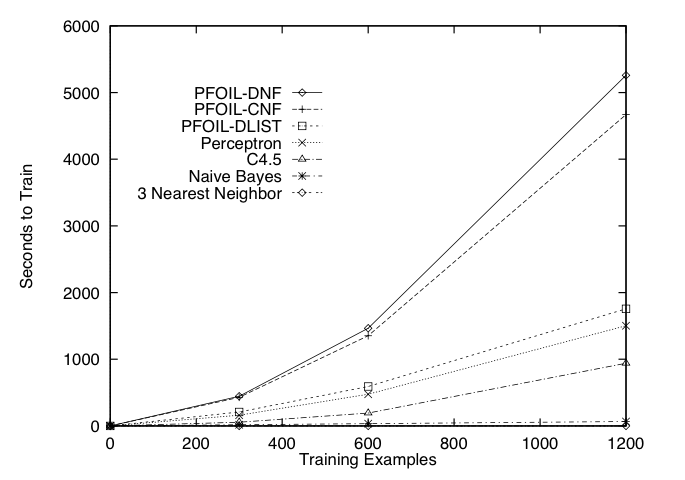
\includegraphics[keepaspectratio=true, width=0.9\columnwidth]{line_wsd_2_time.png}
                \caption{����������� ������� ������������ �� �������� ���������� �� ������� ��������� �������}
                \label{kor2}
        \end{subfigure}%
        \quad% add desired spacing between images, e. g. ~, \quad, \qquad, \hfill etc.
             % (or a blank line to force the subfigure onto a new line)
        \begin{subfigure}[b]{0.48\textwidth}
                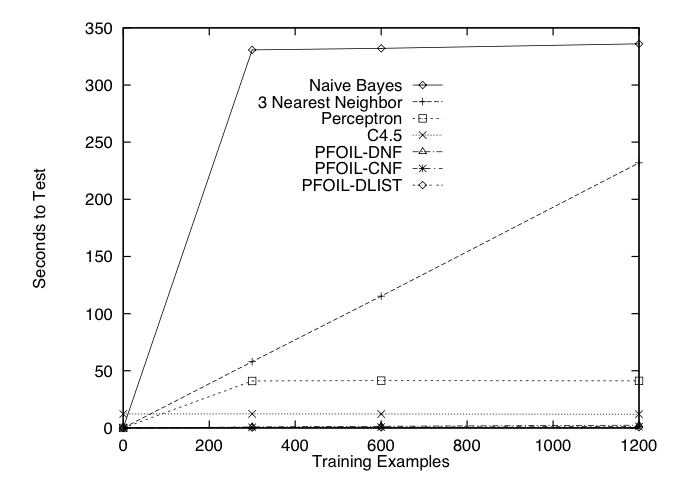
\includegraphics[keepaspectratio=true, width=0.9\columnwidth]{line_wsd_3_testing_time.png}
                \caption{����������� ������� ������ ���������� �� ������� ��������� �������}
                \label{kor3}
        \end{subfigure}%
        \quad% add desired spacing between images, e. g. ~, \quad, \qquad, \hfill etc.
             % (or a blank line to force the subfigure onto a new line)
             
                \begin{subfigure}[b]{0.6\textwidth}
                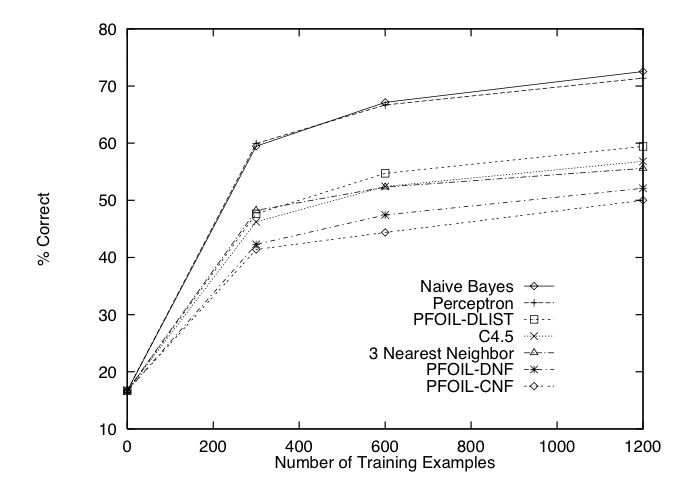
\includegraphics[keepaspectratio=true, width=0.9\columnwidth]{line_wsd_1_accuracy.png}
                \caption{���� �������� ������� WSD-������ ��� ������ ���������� ��� ���������� ������� ��������� �������}
                \label{kor1}
        \end{subfigure}
        \caption{��������� ������� ��������, ������� ������ � ����������� ������ ���������� PFOIL-DLIST, PROIL-DNF, PFOIL-CNF, C4.5, Naive Bayes --- ������� ����������� �������������; Perceptron --- ����������; 3 Nearest Neighbor --- ����� 3-� ��������� ������� ��� ����������� �������� ����� \textit{line}~\cite{Mooney 1996}}\label{figure_alg_comparison}
\end{figure*}

�� ���.~\ref{kor3} ������������ ����������� ������� ������ ���������� �� ������� ��������� �������. ����� ������ ���������� ���� ������ �������: ����������� ������������� � ���������� �������� ����� ��� ������������ ������� ��������� �������, � �� ����� ��� ��������� ������ ������ WSD ������ �� ���������� ����� (���.~\ref{kor3}). 

\bfullwidth
\begin{center}
\section{WSD-методы без учителя}
\end{center}
\efullwidth

\section{���������� �������� ���� �� ������ �������� �������, ����������� ���������� ������������}

\begin{flushright}
\textit{�. �. ��������} 
\end{flushright}

������ ��������� � ��� �������� � 2004 �. ����������� <<�������� ���������� �������� �� ������ ����������� ��������>> (\textit{�ontext vector sense discrimination}) \cite{Purandare 2004}. � ���� ��������� (1) ������� ����� �������� ������������ ������������ �����, (2) ����������� ������������� ���� �������� ���, ����� ������� �� �������� ��� ��������� �����-���� ������� ����� ������������ � ���� ������ \cite{Purandare 2004}.
\parindent=0,5cm

\textit{Word sense discrimination} --- ��� ������ ����������� ���������� ������������ ������� ����� � ��������, ��� ������� �������� ������������� ������������ �������� �������� �����. ������� � ������� ���� �������� ������������ �� �������������� ��������. ������� ��������� ������� \textit{���������� �������� ����} � \textit{���������� ����������� ��������������}. ��� \textit{���������� �������� ����} ��� ������� ���������������� �������� �����, �������������� � ���������; ����� ������ �����, ��������������� � ������ ����������, ������������ � �������� (��������).
\parindent=0,5cm

��� ������� ������ \textit{���������� ��������} ������������ ����������� �������: ���� ������� ����� ����������� � �������� ������, �� �������� ����� ����� �������������� � ���� ������� ���������. \textit{������ ���������} --- ��� ������� ������ �� �������� ������� ������� �� ���� ���������. \textit{������ �������} �������� ���������� � ���������� ������������� ������� ����� � ������� �������, ���� ������ �������� �� ������ ������� ������� �� ����� ��������.
\parindent=0,5cm

����� ���������� �������� ��������� � ��������� \cite{Purandare 2004} ������������ ��� ������ ��� ������������� ������ ��������� ������, ��� ���� ������ ������� ����������� �������, ������������ �� ���������� ��������.
\parindent=0,5cm
���� ����� ���������� � �������� ������� �� �������� ������������ �������� �����.
\parindent=0,5cm

\textbf{���������� ������� ������������� ����.} ������������� �������� ������� ���������� ������������� ���� �� ������ ���������� ������� (���� ������������ ������ Wall Street Journal � ����������� ������������� �������).
\parindent=0,5cm

������ ������� (������ �������) �������� ���������� � ���������� ������������� ������� ����� � �������. ���� ������ � \cite{Purandare 2004}, ��� ����� <<�����������>>, ���� ��� ��������� � ������ �� ���������� �� ����� ���� ������������ (�. �. ����� ���� ��������� �� ����� ���� ����). 
\parindent=0,5cm

\textbf{��������� �������.} ����� �������� ������� ����������� ���������� �������� ������, �. �. ����������� �������� ������������ (����) � ������� ������. ������� ����� � ������� ������������  � �������� ������ ������������� ������ ������� �� ������� �������������. ������� ������ ������� �� ���� ������ ������������� ������� ���������. ����� �������, ����� �������� ������, ���������� ������������ ������������ �����, ������������� � ����� ����������� ��������, ������ �� ������� ������������� ������ �� ������������ �������� �����.
\parindent=0,5cm

���������� �������� ���������� ����� ������������� ����������� �������� � ������� ������������ (partitional) ��� �������������� <<������ ����>> (agglomerative) ��������� �������������  \cite{Jain 1988}, \cite{Jain 1999}, \cite{Zhao 2002}.  ������������ �������� ���������� �� ������������ ������� �� �������� ����, � ������ ������� ������������� ���������� �������� �������� �����. 
\parindent=0,5cm

\textbf{������� �������, ����������� �������� ���������� �� �������.} ������� �������, ���������� �� ���������� ������� �������, ����� ����� ����� ����������� (��������� �����), ��� �� ��������� ��������� ������� �������������� ���������� ������������� ����. ��� ������� ���� �������� ������� ������� ���� ����������� ��������������� ������� (content words), ������������ �� ��������� ���������� ������ �������� ������� �����. � ����.~\ref{tbl2} ������������ ������� ���������� � �������������� ����� ��� ������ �������� ����� <<�������>> �� �������� �����������.

\bfullwidth
\begin{table}[H]
\centering
\caption{��������� ���������� (� �������������� �����) �� ������ ������ <<�������>> �� �������� �����������. ����� ������ � �������� �������� �� �����, ������� ��� ���� � ������� ����, ������~�- ����� ����� �� ����������, �������� ����� �������� ������ �������}
\begin{tabular}{|c|m{10cm}|m{5cm}|}

\hline
� & {\bf ��������} & {\bf �������������� �����}\\
\hline
1 & ������������, ���������������� ��������, ��������� ���������������� & \textit{\textcolor{gray}{��������,}} ���������\\
\hline
2 & �����, ��������� �����, ��������� � �������������� �������� ������������� �������� & \textit{\textcolor{gray}{�����,}} ����, ���������, ��������������\\
\hline
3 & �����, ��������� ��� ��������, ���������������� ��������� �����-���� ������� ������� ��� �������� & \textit{\textcolor{gray}{�����, ��������,}} ���������\\
\hline
4 & ���������������� ��� ��������, ��������� ����-����, ������������ ������ � �������� ������-���� ������� & \textit{\textcolor{gray}{��������,}} ���������, ����\\
\hline
5 & ���������� ����� � ��� ���������, ��������������; ������� & �����, �������, ������������\\
\hline
6 & ��������� �������������, ������� & �������������, \textit{\textcolor{gray}{�������}}\\
\hline
7 & ������� ��� ����������� ��������, ������������, ������ & ��������, ������, ������������\\
\hline
8 & �������, ������������ & �������, ������������\\
\hline
\end{tabular}
\label{tbl2}
\end{table}
\efullwidth

\parindent=0,5cm

�����������, ��������, ��� ������ ������� (������� � ������� �������������) ��� ����� \textit{�������} ����� �������� �������� � �������, ��������������� ������: \textit{�����, ���, �����, �����������, ��������, �������.}
\parindent=0,5cm 

� ������� ����������� ��������� �������� ����� \textit{�������} (����.~\ref{tbl2}) �������� �������������� �����: \textit{�����, ��������������, ���������, �����, ������������, �������������, ������������,} ��������, �������, \textit{��������, �������, ������, �������, ���������, ����.} ����� �������, ������ �������, ��������������� ����� <<�������>>, ����� �������� ������ (�������������� �����) ������� �� �������: \textit{�����, ��������������, ���������, ������������, �������������, ������������, ��������, �������, ������, �������, ���������, ����.}
\parindent=0,5cm

� ����� ������ ������� ����� �������� �����: \textit{�����, ��������������, ���������,} �����, ���, �����, \textit{������������,} �����������, \textit{�������������, ������������,} ��������, �������, \textit{��������, �������, ������, ���������, ����.}
\parindent=0,5cm

��� ������ ����������� ���� ��������� ������ �������� �������� � �������� ��������. �������� ������������� �� ��������, �������� ������������ �������� � ��� ���� ������ �����. 
\parindent=0,5cm

�������� ���� ��������� 75 ������������� � �������������� 72 ���� �� ������� SENSEVAL-2 � �� ������� \textit{line, hard} � \textit{serve.}
\parindent=0,5cm

� �������� ������ SENSEVAL-2 ������� ������������ �������� 2--3 �����������. ��� ������� ����� ���� ���� �� 50 �� 200 �������� ������������ � �������� � ������������� ������. ��� ���� ���� �������� ����� (������� 8--12) ��������. ����� ����� �������� ��� ������� ����� �������� ������� � ����, ��� ��� ��������� �������� ��������� ���� �������� ������������. 43 �� 72 ���� SENSEVAL-2 �������� ��������� F-���� � ������� (recall) ��� ���������� ������� ������� �������� ���������� �������. ������ ��� 29 ���� F-���� ����� ����, ���, ��������, ������� � ������������ ���������� ������, � ��� ����� � �������������������� �������. ��� ������������� ������ ���������� ������� ����������������� ����: �� ������� ����, � ������� � ����� �����.
\parindent=0,5cm

������ ����� ����� ���� ������� ��� ����������  �������� ���� ��� ������� ��� ��������� ���������� ��������� ������.


\section{�������������� ����� � ������������� ������� ����}

\begin{flushright}
\textit{�. �. �����} 
\end{flushright}

� ������ \cite{Dekang 1998} ����������� ����� ��������������� �������� ���������, ���������� �� ������� ������� ������ � ���������� �������� ����, �������� �� ��������. �������� ����������� ����� ����� ����� ���������� �� ��������� \cite{Eugene 1975}.  ����������, ��������, ��������� �����:
\begin{flushright}
(1)\textit{������� Tezg\"uino ����� �� �����. ���� �������� Tezg\"uino. Tezg\"uino ����� �������� � ���������. �� ������ Tezg\"uino �� �����.} 
\end{flushright}

�� ����� ��������� ����� ������������, ��� \textit{Tezg\"uino} --- ��� ����������� �������, �������������� �� �����.

������ ������ ������� ���� \textit{(similar words)} �������� ������ ����� � ����������� �������� �����. ����� ��� ��������� �������, ����������� ����������� (1), ����������� ������ ���� ����������� �������� �������� ����� \textit{Tezg\"uino} � ������ \textit{����, ����, �����.}

\textbf{����������� ��������������� �������� ���������.} ��� ���������� �������� ����� ������� � ������ \cite{Dekang 1998} ����������� ������ \cite{Dekang 1993}, ����������� ������ �� ������. ������ ������������ (�� ����. \textit{dependency triple}, ����� ������ \textit{������}) ������� �� ���� ���� � ��������������� ��������� ����� ����. ������ $||w, r, w'||$ �������� ������� � ������� ������ $(w, r, w')$, ��� $w, w'$ --- ��� ����� � ���������� �����, $r$ --- �������������� ���������. ������������ ����� ��� ��������� ������������ ��������-�������� �*�. ��������, ||\textit{cook, obj,} *|| �������� ����� ����� �� ������ \textit{cook} � ���������� \textit{obj}. 

�������� �� ����������� \textit{<<� ���� ���� ���������� ������>>} ����� ��������� ��������� ������:

\begin{center}
||\textit{����������, ����\_���, ������}||\\
||\textit{����, ��\_���, ������}|| 
\end{center}

��������� ��������� �������:
\begin{enumerate} 
\item \textit{�������� ����� w} --- ��� ������� ���� ����� ($w$, *, *) � �������,  �� ���� ���� �����, ���������� $w$. �������� ����� $w$ �������� ��������.
\item \textit{<<�����������>> ���� ����} --- ��� ������, �������������� � �������� ����� ����; ��� ����������� ��������.
\end{enumerate}

�������� ����� ����� ��������� ����������� ��� ���������� ���������� � <<�����������>> ���� �������� (2), �������� �� ���������� ���������� � �������� ���� �������� (1), ����� ���������� ��� ������� \textit{sim($w_1, w_2$)}~\cite{Dekang 1997}.

�����������, ��� ������� ����� �� ������� ���� �� �����, ��������, ��� ����������, �������������� � �������� ����� $w$, ����� ����� ���������� �� ������ �� ���������� ����� � �������� ����� $w$. 

��� ��������� ���������� � ����������� ||\textit{w, r, w'}||\textit{=�} �������� ���������:

\begin{enumerate}
\item ������� ���������� ���������� � �����������, ��� ������������ ������, ����������� �� ������, ����� ���� ������ \textit{(w, r, w')} ��� �������, ��� �������� ||\textit{w, r, w'}|| --- �� ��������;
\item ������� �� �� ��� �������, ��� �������� ||\textit{w, r, w'}|| --- ��������;
\item ������� ���� ���� ��������� �������� �������.
\end{enumerate}

����������� ��������� � ������ ������ \textit{(w, r, w')} ����� ������������� ��� ������������� ������������� ���� �������:

\textbf{A:} �������� ��������� ����� - ��� $w$;

\textbf{B:} �������� ��������� ���������- ��� $r$;

\textbf{C:} �������� ��������� ����� - ��� $w'$;

\begin{enumerate}
\item ����� �������� ||\textit{w, r, w'}|| ����������, �� ������������, ��� \textbf{�} � \textbf{�} �������� ������� ������������ ��� ������� ������� \textbf{�}.  ����������� ����������� ����� ���� ���� ������� ���������� \textbf{$P_{MLE}(B) P_{MLE} (A|B) P_{MLE} (C|B)$}, ��� \textbf{$P_{MLE}$} --- ��� ������ ������������� ������������� ������������� ������������ (\textit{maximum likelihood estimation})

$P_{MLE}(B)=\frac{\displaystyle ||*,r,*||}{\displaystyle ||*,*,*||}$\\
$P_{MLE}(A|B)=\frac{\displaystyle ||w,r,*||}{\displaystyle ||*,r,*||}$\\
$P_{MLE}(C|B)=\frac{\displaystyle ||*,r,w'||}{\displaystyle ||*,r,*||}$

\item ����� �������� ||\textit{w, r, w�}|| ��������, ����� ����� �������� $P_{MLE}(A,B,C)$:

$P_{MLE}(A,B,C)=\frac{\displaystyle ||w,r,w'||}{\displaystyle ||*,*,*||}$
\item ����� \textit{\textbf{I(w,r, w�)}} ���������� ���������� ����������, ������������ 
� ����������� ||\textit{w, r, w'}||\textit{=�}. ����� ��������� ��� �������� ���:
%
\begin{multline*}
I(w,r,w�)= \\
=-log(P_{MLE}(B) P_{MLE} (A|B) P_{MLE} (C|B))- \\
-(-log(P_{MLE}(A,B,C))= \\
=log\frac{||w,r,w'||\times||*,r,*||}{||w,r,*||\times||*,r,w'||}.
\end{multline*}
\end{enumerate}

�������, ��� �������� \textit{I(w,r,w�)} ����� ���������� �������� ���������� (\textit{mutual information}) ����� $w$ � $w'$ \cite{Donald 1990}.

����� $T(w)$ --� ��� ��������� ��� \textit{(r, w')}, ��� ������� $log\frac{\displaystyle ||w,r,w'||\times||*,r,*||}{\displaystyle ||w,r,*||\times||*,r,w'||}$ ����� ������������� ��������. ��������� �������� �������� (���������) ���� ���� \textit{w1} � \textit{w2} � ������� �������:

\begin{multline*}
sim(w_1,w_2)= \\
\frac{\displaystyle \sum_{(r,w)\in T(w_1)\cap T(w_2)}(I(w_1,r,w)+I(w_2,r,w))}{\displaystyle \sum_{(r,w)\in T(w_1)}I(w_1,r,w)+\sum_{(r,w)\in T(w_2)}I(w_2,r,w)}.
\end{multline*}

\textbf{������������ ���������� ������.} ��� ��������� ������, ���������� 64 ���. ����. �� ���� ���� ��������� 56,6 ��������� �����, ���������� 8,7 �������� ���������� �����.

��� ������ ��� ������ �� ������ �� ������ ����.  ������������� ������� �������� ����� ����� ���������, ����� ����������������, ����� ���������������/��������� �� ������� $sim(w_1 , w_2)$. ��� ������� ����� ��� �������� ������ ��������� ������ � ���������, ���������� ������������� ����� 200 �������� ������� ����. ������ � ��������� ��� ����� $w$ ����� ��������� ������:\\

$w(pos):w_1,s_1,w_2,s_2,\ldots,w_N,s_N$\\

��� \textit{pos} --� ��� ����� ����, $w_i$ ---  ��� ������� �����, $s_i$ --- ��� �������� �������� ����� $w$ � $w_i$, ����� ����������� �� �������� �������� ��������.

��� ����� �������� \textit{����� �������� ��������� ������� (RNN �� respective nearest neighbors)}, ���� ��� �������� �������� �������� ������� ���� ��� ����� (������� � ������ �� ������� ����). � ������� ��������� ������� �������� 543 ���� RNN ���������������, 212 ��� RNN ��������, 382 ���� RNN ��������������/������� � ��������� ������������� ���������. � ����.~\ref{tabshor} ����������� ������ ������� 10-�� RNN ��� ��������.

\begin{table*}
\centering
\caption{������ ��� �������� ��������� ������� (RNN) ��������}
\begin{tabular}{|c|c|c|}
\hline
\textbf{����} & \textbf{RNN} & \textbf{�������� ��������}\\
\hline
1 & \textit{fall rise} & 0,67\\
\hline
11 & \textit{injure kill} & 0,38\\
\hline
21 & \textit{concern worry} & 0,34\\
\hline
31 & \textit{convict sentence} & 0,29\\
\hline
41 & \textit{limit restrict} & 0,27\\
\hline
51 & \textit{narrow widen} & 0,26\\
\hline
61 & \textit{attract draw} & 0,24\\
\hline
71 & \textit{discourage encourage} & 0,23\\
\hline
81 & \textit{hit strike} & 0,22\\
\hline
91 & \textit{distregard ignore} & 0,21\\
\hline
101 & \textit{overstate understate} & 0,20\\
\hline
111 & \textit{affirm reaffirm} & 0,18\\
\hline
121 & \textit{inform notify} & 0,17\\
\hline
131 & \textit{differ vary} & 0,16\\
\hline
141 & \textit{scream yell} & 0,15\\
\hline
151 & \textit{laugh smile} & 0,143\\
\hline
161 & \textit{compete cope} & 0,136\\
\hline
171 & \textit{add whisk} & 0,130\\
\hline
181 & \textit{blossom mature} & 0,12\\
\hline
191 & \textit{smell taste} & 0,11\\
\hline
201 & \textit{bark howl} & 0,10\\
\hline
211 & \textit{black white} & 0,07\\
\hline
\end{tabular}
\label{tabshor}
\end{table*}

\section{������������� ����������\\ �������������� �������}
\begin{flushright}
\textit{�. �. ��������} 
\end{flushright}

� ������~\cite{Savova 2005} ��������� ������ ������������� ��� ������� � �� ������������� ��� ������� ����������� �������������� ��� ��������� ������� �� �����������. ������� \mbox{�������} ����������� �������������� � ������ ������� �������� � ���� �� ������ ������������ ������ ���������� ����� ������������ ��������� �������� ��� ��������, �� ����� � ����������� ����� �������� ��� ���.

��� ���������� ����������� �������������� ������ � ��.~\cite{Savova 2005} ����������
��������� ��������� (��������� ������), ���������� ������������ ������� �����, �� ��������, ��� ������ �������� ����� ��������������� ��������� ��������� �������� �����. ������ ������� ������� �� ������� �� �������� ����������. ��������������, ��� ������������ ������� ����� � ����������� ��������� ����� ����� ���� � �� �� ��� ����� ������� �������� (�������������� ��������).

������� ������������� ������������ �� ��� ���, ���� �� ����� ������� �������������� �������� ����� ���������. ����� ����� ��������� � ������~\cite{Savova 2005} ������� �� ��� �����, ��� ��� ������, ��� ������������ ����� ��������� �������� ������ ����������� �����, ����������� ����� ������ (����������� ���� ����� ���-��� ��������). ������������ ������ �� �����������.

������ � ���� ������������ ������� �� ���� ����������, ������� �������� ������ ������� �����, ��� � ������� �������� ����� ������� ��������, ����� �������� �� ������� ���� ������������ � ���� ���������. ��������~-- ��� ������������ �������� ���������� � ������� �����. ���� ������������~-- ������������� �������� � ����������� ������� ������� � ������� ������� \cite{epr:website}. ����������� ������� �������� ��������� ������������ ��������: ��������, ���������� ������������� � ���������� ������������� �������� �����. ���������� �������� ��� ����������� ��������������, ��� � ����� ��� �����, ������������� ����� � ��������� ������. ��� ��������������� ������������ ����� ���� ������� ������ ������������� ������ ������� \cite{Averin 2006}. 

����������������� ������~-- ��� ����� NLM WSD \cite{UMLS:website} (NLM~-- ������������ ���������� �������� ���), � ������� �������� ���� ����� �� UMLS (������ ������� ����������� ������������). UMLS ����� ��� ���� ������: 
\begin{itemize}
\item {\it ������������} �������� ��� ������� �� �������������� �������� (SNOMED-CT, ICD � ������) � �������, ������� ������������ ����� �������� �� ��������, ����������� ���� � ��� �� �����. 
\item {\it ������������� ����} ������������ ������� �� 134 ��������� � ���������� ��������� ����� ����. SPECIALIST-�������� �������� ������������� ���������� ��� �������� �������������. 
\item {\it Medline}~-- ������� ����������������� ���� ������ NLM, ������� �������� �������������� 13 ��������� ������ �� ���������� ������ � ������� ����� � ����� � ������� � �������������� \mbox{�������}.
\end{itemize}

������ ������� ��������� �� ��� ������������ ������������ ������� (PB~-- Pedersen and Bruce \cite{Pedersen 1997}, SC~-- Sch\"utze \cite{Schutze 1998}) � ������� ������������� ������������� SVD (����������� ���������� ������). ������ PB �������� �� ����������� �������� ������� ������� -- �������� �������������� ����������� �������� ����� ��� ��������. �������������� ������� ���������� ����� ���������� ��� �����������  ����� ��������. PB~������ �������� ��� ������ � �������� �������� �������� ������. ������ SC �������� �� �������������� ������� ������� -- ������� ��������� �������������� ����������� ��� ��������, ��� ������ ������ � �������~-- ������ ��������� ������� ������� ������� �����. ��� �� �������������� ������� ���������� ����� ���������� ��� �����������  ����� ��������. SC ������ �������� ��� ��������� ��������� ������� ������.  

����� SC2 (�������� �������������� ����������� ������� �������, ������� ���������� ����� ���������� �������� � ������������ �������) � ����������� � ��� SVD ������� ������ ����������: ����� 56 ������������ �����������, � 47 ������� ����� SC2 ������� ��������� ����������, � 7 ������� ���������� ������������� ���������� �� ������ ����������� �������.

��� ������������, ��������� � ������������, ����������� � ������� ������ SenseClusters \cite{SC:website}. � ���� ������������ ���� ��������� ��� ������������ ��� ������ ������� ������. ��������� ������������� ����� -- ��� ����� NLM WSD, ������� �������� 5000 ����������� ��� 50 ����� ����������� ������������� �������� �� ������������� UMLS. ������ ������������� ������ ����� �� 100 ����������� � ��������� ������� ���������. � 21 ������� ������������ ����� ����������� ��������� � �������� �� 45 �� 79 �����������. � 29 �������� ����� ����������� �� 80 �� 100 ���  ����������� ��������. ����� ��������, ��� ������ ������ ����� ��������� ��� ���� �� ���������������, ������� ���������� ��� ���������� ��������, �� ��������������� ��������� � UMLS. ������� ������������� ����� �������� �������������� �1999 Medline�, ������� ��� ���������� Weeber \cite{Weeber 2001}. ���� ���������� ��� ����� �� ������ NLM WSD � ������������ � �������� �1999 Medline�. ��� �������� �������������� ������ ����������� �������������� ������ �� ������ �� �1999 Medline�, ������� ���� ������� ������������ � ������ NLM WSD.

������������� ������� ������ ��������� ������ � �������� ��������� �������� � ������ �����������, ��� ������������� ��������� �����������. � ����� �������, ������� ����� ���������, �������������� ����������, ���� ������� ��������� ���������, � ������ �������, � ��������� WSD ������������ ��������� ����� ����������.



\bfullwidth
\begin{center}
\section{WSD-методы, основанные на знаниях}
\end{center}
\efullwidth

\section{��������� �������� ���� �� ������~--- ������������� ����������� ���������}
\begin{flushright}
\textit{�. �. �������} 
\end{flushright}

� ������ \cite{Pantel 2002} ����������� �������� ��������������� ����������� �������� ���� � ������, ��������� \textit{������������� ����������� ���������} (Clustering By Committee, ����� CBC). ����� ������ ���������� ����������� ������ ��� ��������������� ��������� �������� � ������� ��������� ��������.

\textbf{��������} ������������� ������� ��������� ���������� ���������, ���������� ����������, ������ �� ������� ������������ ����� ���� �� �������� ������������� �����. ����� �������  ������ �������� (���� ��������� � ������������ ������) ������������ � �������� ������� ��������� ��������.

�������� CBC �������� ��� �����.

\textit{�� ����� I ��� ������� �������� (�����) ����������� $k$ �������� ������� ����, �������� ���� ������ �������� $S$}. ������� ���� ������ ����������� � ����� �������� ����������� �� �������� �������� ����� �������� �������� PMI (�������� �������� ����������, pointwise mutual information~\cite{Manning 1999}, �.~66--68), � �����, � ������� �������������� ����������� ������� �� \textit{������ ������� �����} \cite{Kim 1989}, ����������� �������� ����� ����� ���������� �������� �������. �������� ������� PMI ����� �������������� ��������� ����� (����������) � ��������� (������) ����������� ��������� �������: ����� $x$ --- ��� ��������������� �������, � $y$ --- ��������. \textit{�������� �������� ����������} ����� $x$ � $y$ ���������� ���:

$$
pmi(x;y)\equiv log \frac{\displaystyle p(x,y)}{\displaystyle p(x)p(y)}=
$$
$$
=log\frac{\displaystyle p(x|y)}{\displaystyle p(x)}=log\frac{\displaystyle p(y|x)}{\displaystyle p(y)}.
$$

\begin{algorithm*}
\SetAlgoLined
\KwData{$(E, S, \theta_1, \theta_2)$, ���  $E$ --- ��� ������ ���������, ������� ����� �������������, ���� ������ �������� $S$ (��������� � ���� ����� I), ������ $\theta_1$ � $\theta_2$ (� ������� ������ $\theta_1$ ����������� ������ �� ��������, ������� ����� ��������, �������� �� ����� ������������, ����� $\theta_2$ ��������� ���������� ��������, �� ������������� �� ������ �� ���������)}
\KwResult{$C$ --- ������ ���������}
\textbf{Step 1:}\\
\ForEach{$e \in E$}{\begin{enumerate}
\item ������� $k$ �������� <<�������>> (�������) ��������� $e$ �� $S$ � ������� ������  \newline ������� �����.
\item ��� ������� ������������� �������� $c$ ��������� ��������� ������:
$val = | C | \times avgsim(c)$, ��� $| C |$ --- ���������� ��������� $c$ � $avgsim(c)$ --- ����������� �������� ����� ����� ������ ��������� �������� $c$.
\item �������� ������� � ��������� ������� � ������ $L$.\end{enumerate}}
\textbf{Step 2:}\\
SortByDecreasingOrder$(c(val) \in L)$ // ���������� ��������� � ������ $L$ � ������� �������� �� ������ $val$.\\
\textbf{Step 3:}\\
$C = \emptyset$ // �����  �������� ��������� $C$ ����� ���������� ������.\\
\ForEach{$c \in L$}{// � ��������������� �� �������� �������:
\begin{enumerate}
\item ��������� ����� �������, �������� ����������� �������� ��������, � ��������� 
\newline ������  PMI ��������� (��� ��, ��� � ��� ��������� ��������� �� ���� 1).
\item ���� �������� $c$ � ��������� ������� ��������, ����� ������������ � $C$, ���� ���������� $\theta_1$, �� ������� �������� $c$ � $C$.
\end{enumerate}}
\textbf{Step 4:}\\
\If{$C=\emptyset$}{\Return $C$}
\textbf{Step 5:}\\
$R = \emptyset$ // $R$ --- ��� ��������� ��������, �. �. ���������, �� ���������� �� ����� �� ���������\\
\ForEach
{$e \in E$}
%{\ForEach
%{$c \in C$}
{\If{$sim(e,$ foreach  $c \in C) < \theta_2$ //  �������� �� ���� ��������� �� $C$ ������ $\theta_2$ // }
{$R += e$ // �� ������� �������� $e$ � ������ �������� $R$.}
%}
}
\textbf{Step 6:}\\
\If{$R=\emptyset$}{\Return $C$ \Else{\Return $C \cup Algorithm1(R, S, \theta_1, \theta_2)$}}
\caption{���� II. ����� ���������}
\label{alg_phase2}
\end{algorithm*}

\begin{algorithm*}
\SetAlgoLined

\KwResult{�������� �������� � ������������ ��������� ����� $val$ ����� ������� (��. ���������� $val$ �� ���� 1 � 3 ���������~\ref{alg_phase2})}
����� $C$ --- ��� ������ ��������� (���������� ������).\\
����� $S$ --- ��� ������ 200 ���������, �������� ������� �� $e$ (���� ������ �������� $S$ ��������� � ���� ����� I).\\
\While{$S\neq\varnothing$}{����� $c \in S$ �������� ������� ������� � $e$\\
\If{�������� $(e, c) < \sigma$}{\textbf{����� �����}}
\If{$c$ �� ���� �� � ����� ��������� � $C$}{��������� $e$ � $c$;\\
������� �� $e$ ��� ��������������, ������� ������������� � ���������������� $c$;}
������� $c$ �� $S$
}
\caption{���� III. ���������� ��������� ���������: ��� ������� �� ��������� $e$ ��������� �������� ������� �������, � �������  ���������� $e$}
\label{alg_phase3}
\end{algorithm*}

��� ������������� ����������� ������ ������� ������ \textit{(average-link clustering)} ����������� ������� �������� ����� ������ �������� � ����� ��������� � ��������, � �����, ���� ��������� \textit{������� �������� ��������} ��������� ��� ����������� ��������� �������� ��������� ������� ��������, ������ �������������� � ����� �������� \cite{Kim 1989}. ��������� ����� ��������� $O(n^2 \times  log (n))$, 
��� $n$~-- ����� �������������� ��������� \cite{Jain 1999}.

�� II ����� ��������~\ref{alg_phase2} ���������� ������ ����� ���������� ���������, ��������� ���� �� �����, ��� �������� ������� �������� �������� �������. � ���� ������ ���������~\ref{alg_phase2} ����������� ��� ����� ������ ��������� ��� �������, ��� ������ ����� ��������� ������� �� ������� ����� �� ����� �� ��� ������������ ���������. ���� ������� ����������, ������� ������ �������������.

�� ������ ����������� ������ ��������~\ref{alg_phase2} ������� ���������� ����� ��������� (�� � ��������  ����������) � ���������� ���������� ��������, �� �������� �� � ���� �� ���������. ����� ��������, ��� ������� <<���������>> ������� (��� ������� <<������>> � �������), ���� �������� �������� ����� ��������� � ���������� �������� ���� ��������� ��������� ��������. ��� ��������� ����������� ������ �������� ����� ���� �������� ����� ���������� ���������. �� ������ ��������~\ref{alg_phase2} ���� ������ ���� ��������� ���������.

�� ���� 1 ���������~\ref{alg_phase2} ������ ��������� ������������ �������� ������� � ���������� ���������.
�� ���� 2 �������� ����������� �� �������� �������� ��� ������������ ������ ������� ��������.
�� ���� 3 ������� ����������� ������ � ��� ������, ���� ��� �������� �� ����� ����� ����������� ���������� ���� �������������� ���������� �������� (� ������������� ���� �������� �������� $\theta_1=0,35$).
�� ���� 4, ���� �� ���� ������� ��������� �� ���������� ����, �������� ���������������.
���������� � ������ �� �������� �������� (�������) ������������ �� ����~5. ���� ����� �������� ���, �� �������� �����������, �����~-- �������� ���������� ���������� ��� ��������.

� ���������� ������� ����� ���������� CBC �������� ������� ���������� �������� (������� �\'������ �������� $val$, ��. ���� 1 � 3 ���������~\ref{alg_phase2}), ������ ������������ ���� �� �����. �� ������� ����� ��� �������� �������������� �� ���� ���������, � ������: ������ ������� $e$ ������������� �������� �������� ��������, ��� ���� �������� ������ �������� ������������ � �������� ������� ������������� �������� (��������~\ref{alg_phase3}). ��������� �� ����������, �. �. ��� ���������� �������� � ������� ������� �� ����������� � ������� ��������.

�������� CBC ���������� �� �������������� ��������. 
�������� CBC ��������� ����������� ��������������, ��������� ����� �������� �������� �� ����������. ������� ����������� �������� ������������� ���� �� �������� �����.

%� ����.~\ref{yank} ������ ������ ���������� ��������, ������� ����������� ��������� �����. ����� ��� ��������� Nq34, Nq137, $\ldots$ ������������ %�������������. ����� ������� ����� �������� ��������� �����, ������������ �������� ����� ��������� � ��������� ������ (�.�. �����, ������ � ������). %����� ������������� ������ �����, �������� ������� ��������� ��������. ������ ������� ������������� ������ �������� ���������� �����. ��������, Nq34 %������������� �������� <<������ ������>>, � Nq137 ������������� �������� <<����������� ����� ����>>.

%\begin{table}[H]
%\caption{��� ���������� ��������� �������������� ������ ��������� ������ �����������: <<������>>,  <<�����>> �  <<������>>}
%\begin{tabular}{|c|c|m{5cm}|}
%\hline
%\multicolumn{3}{|c|}{�����}\\
%\hline 
%Nq34 & 0.39 & ������, �������, �������\\
%Nq137 & 0.20 & �������, �����, ������, �����\\
%Nq217 & 0.18 & �����, �����, ������������\\
%\hline
%\multicolumn{3}{|c|}{������}\\
%\hline
%Nq72 &  0.27 & �����, ������� ����, �����\\
%Nq866 & 0.17 & ����, ��������, ��������\\
%\hline
%\multicolumn{3}{|c|}{������}\\
%\hline
%Nq215 & 0.41 & �����������, ����, �����\\
%Nq235 & 0.20 & ��������, ��������, ������\\
%\hline
%\end{tabular}
%\label{yank}
%\end{table}
%
%� ����.~\ref{yank} ������ ������ ���������� ��������, ������� ����������� ��������� �����. ����� ��� ��������� Nq34, Nq137, $\ldots$ ������������ �������������. ����� ������� ����� �������� ��������� �����, ������������ �������� ����� ��������� � ��������� ������ (�.�.  {\it �����}, {\it ������} � {\it ������}). ����� ������������� ������ �����, �������� ������� ��������� ��������. ������ ������� ������������� ������ �������� ���������� �����. ��������, Nq34 ������������� �������� <<������ ������>>, � Nq137 ������������� �������� <<����������� ����� ����>>.

\textbf{��������� � ���������� UNICON.} CBC �������� �������������� ��������� UNICON \cite{Lin 2001}, ������� ����� ������ �������� ��������, ��������� ��������� ����� ������� ���������.

����� �� �������� �������� ����� UNICON � CBC �������� ��, ��� UNICON �����������, ��� ��������� �������� �� ����� ���������� ���������, ��� �� ����� \mbox{������} ������� ���� ��������� ��-�������� ����� ���� ����� �������� (��������). �~UNICON'� ��� �������� �������� ������������ ����� ���������. � ������� �� ����� �� II ����� CBC ��������� ������ �� \mbox{��������}, ������ ������� ������� ������� �� ���� ����� ��������� ���������.

���� ������� � �� III ����� CBC. �������� UNICON ����� �������� �� �������, ������� ����� ��������� ������ ������������ (������������) ��������. 
%��������, ����� �������� <<�������>> �������� ����� ����������� ��� ����� <<����>>, ��� �������� <<������ ��������>>. �������� ����� ������ ����-��������� ��� ������ �������� ����� <<����>>: ����������, �����������, ������, ��������, ��������, �������, ���������, ������, ��������, �����������, �������, ����, ����������, �������, ����������, ����. � ���� ������ 10 �������� ��������� � �������� <<�������()>>, 4 � <<������ ��������()>> � 2 � �������� <<����()>>. �� ����� ������ ���������� UNICON ����� ������������� �������� <<�������>>, <<����������>>, <<�������������>>,<<������������>>, <<������>>, <<������ ��������>>,<<�������������>>, <<�����>>. �������� ����� ������ � ����������� ����������  �������� ����� ������, � ���� �� ���� ��������, ���������� ���������� �����. 
%� ������ �������, 
CBC ������� <<��������������>> (����� ��� ���� ���������) �������������� (�����) ����� ����, ��� �������� �������� ��������.
%(��������, ��������������, ����������� � �������� <<�������>> ����� <<����>>, ����� ������� �� ������� ������������� <<������ ��������>>). 
%� ���������� �������� �����  ��������� <<������ �������� (������, ��������, ��������, �������)>> � �������������� �������� ������������� �������� <<������ ��������>> ���������� ������� ����. ���, � ���� �������, 
��� �������� � ����, ��� �������� ������ ������������� ������� ���������.

\section{������������� ����������� ������� ��� ������������� �������}
\begin{flushright}
\textit{�. �. ���������} 
\end{flushright}

� ������ \cite{Barzilay Elhadad 1997} � ����� ������������� ������ �������� ������ � ���� ����������� �������. ������������� �������� ������ �����: ������������ ����� ������� �� ����� (��������), �������� ����������� �������, ������������ ������� �������, ����������� ������ �����������.

�������������~-- ��� ������� ������ ��������� ������ � ����� ���������� ��� ���������� ��������������� ������. ������������� ����������� ��� ������� ������ �����~-- �� ��������� ������� ������� �����-���� ������� ������� �� �������� ��������� ������� ��� ������. �������� ������������ ������������� ��������� ������������� ������ �������� ������� �������, ��������� ������� ��������� ������. ����� ���������  ���������������, ������������ ��������� (indicative summaries), ����������� ������� �������~-- ����� �� ������ �����. � ������ \cite{Barzilay Elhadad 1997} ������ ����� �������� ������������ ��������� �� ������������ �������.

����������� ������� \textit{cohesion} (���������, ����������, �������), ��������� � \cite{Halliday Hasan 1976}, ��������� �� ����������� ������ ������ (����������) ������ � ���� �����, � ��, ��� ����� ��������, �����. ����� �� ����� ��������� �������� \textit{����������� ���������} (lexical cohesion) \cite{Hoey 1991}. ����������� ��������� ����������� � ������� ������������ ��������� ����. �������� � ����� \cite{Halliday Hasan 1976} ��������  ��� ������� ������������ ����������� ���������: (1) � ������� ��������� ���������� � (2) ��������� ��������������. 

\begin{enumerate} 
\item \textit{����������� ��������� ����������} (reiteration category) ����������� �������� ����, �������������� ��������� � ���������. 
\item \textit{����������� ��������� ��������������} (collocation category) ���������� ��� ����, ������� ����� ������������� ������, �. �. ����������� � ����� � ��� �� ����������.
\end{enumerate}

����� � �����, ����� �������� ���������� ����������� ���������, ��������� ����������� ������� (lexical chain)~\cite{Hoey 1991}. ����� ����������� �������, ������������ �������� � ��������~\cite{Barzilay Elhadad 1997}, ������� �� ������� ���������� ������������� ���� � ����������� ������ ����� �������. 

\textbf{�������� ���������� �������.} ����������� ����������� ������� � ���, ��� �� ����� ���������� � ���������. ������ �������������� ������ ��� ����������� ������� ���� ������������ � ������ ������� � ������~\cite{Morris Hirst 1991}. ������� ����������� ����� ������ ������ ����� �� ������ � ������ ����������� (���������) ������� ��� ����� � ������������ � ���������� �������. ����������� ������� �~\cite{Morris Hirst 1991} ���� ��, ��� � ���� ������� ����� ������� ����� � ������� ���������� (��� ������������ ����). ����� �������, ����� ���������� ������� ��� ����� ������������ ������� WSD-������.

����� ���������� ����������� ������� �������� ����:

\begin{enumerate} 
\item ���������� ����� ����-���������� (��������������� � ��������� ���������������). ��� ��������� �� ��������� � �������.
\item �������� ������ ���� �������� ��� ������� �����-��������� (�� �������).
\item ��� ������� �������� ������� �����-��������� ��������� (�����������) ��������� (����������) �� ������� ����� �� ���� ��� ����������� �������� (����� � ������� ����� ������ ������������ ��������, ���������� ������� ������� � ��� �� �������). ����� ����� ������� ���� ��������� (����� ������� ����� � �������), ���� ���� ���������� ����� ����� ������� � ������ (text distance) ��� ����� ���������� ���� ���� ���������� ���� � ��������� WordNet. �������� ��� ���� ��������� \cite{Do Thuy Duong 2011} (�. 36):
\begin{enumerate} 
\item \textit{Extra-strong} ��������� ���������� ��� ����, ������������� � ������. ������ ����� ���� �� ����� ���������� �� ������� ������������ �����.
\item \textit{Strong} ��������� ���������� ����� �������, ���������� ���������� � WordNet. ��� ����� ����� ������ ���������� � ���� �� ����� ���� �����������.
\item \textit{Medium-strong} ��������� ����������� ��� ����, ������� ������� ��������� �� ���������� ������ ������ � WordNet (�� ���� ��� � �������������� ����������� �� ���� ����� ���������). ����� � ������ ������ ���������� � �������� ���� �����������.
\end{enumerate} 
\item �����-�������� ����������� � �������, �� ������� ������� ������� �����. ��������� ��������������� �����������, � ������� ����������� �� ������ �����, � ��� ���������� �������� (��������� ������ �������� � ������� �� ���� 2).
\end{enumerate} 

��� ������ ������������ ������� (��� ������� �����-���������) ��������� ����������� ���: extra-strong, strong, medium-strong. � ������ ������ � ��-��� \cite{Hirst St-Onge 1998} ��������� ������ �������� ������ �������. ��� ���� �����-�������� �������� ����� � ���� ������� � ����� ����� ����� ��� �� ����� ���� �������, ���� ���� ����������� ����� ������� ����������� ��������������� �������. � ������ �������� � �������� \cite{Barzilay Elhadad 1997} ���������� ����� ������� ����� ������ <<����������� ��������>>, ��������� ������������ ���� ��������� �������. ����� �������, ����� ������������ ������� � ������ ���� ��������� �������� ���� � ����������� ������� ��������� �������. ��� ����� ������� ����� � ��������������� �����.

��� ����������� ������ ���������� ������ �� ������� ������, �������������� ����, ���������, ����� �������� ����� ������� ��� ����� \textit{machine}. ��-������, ��� ����� \textit{Mr.} ��������� ���� [������� <<Mr.>>, �������� \{\textit{mister, Mr.}\}]. ��������� �� ������ ���������������, �������������� � ��������� WordNet, ����� ����� \textit{person}, � ���� ���� ��� ��������: [������� <<person$_1$>>, �������� \textit{\{human being\}}] � [������� <<person$_2$>>, �������� \textit{\{grammatical category of pronouns and verb forms\}}]. ������� ���� �������� � ����� \textit{person} ��������� ������������ ������� �� ��� ��������� �������������: � ������ ������������� ������������ ��������  $person_1$, �� ������~-- $person_2$ (���.~\ref{step1}).
%\textit{<<human being>>} ($person_1$) � \textit{<<grammatical category of pronouns and verb forms>>} ($person_2$).


\textit{\textbf{Mr.} Kenny is the \textbf{person} that invented an anesthetic \textbf{machine} which uses \textbf{micro-computers} to control the rate at which an anesthetic is pumped into the blood. Such \textbf{machines} are nothing new. But his \textbf{device} uses two \textbf{micro-computers} to achieve much closer monitoring of the \textbf{pump} feeding the anesthetic into the patient.}

\textit{�����������} � \cite{Barzilay Elhadad 1997}  �������� ������ \mbox{�����������������} �������������. ������ \mbox{�����������} ��������� ����� ������ �� �������� ���� ����� � ������ ��������������� �������������, � �������������, � ������������� ������ ������������� �� ���� ����������. ������������� 1 � 2 �� ���.~\ref{step1} �������� �����������.

��������� ����� \textit{anesthetic} �� ������� �� ������� �� ������ ����������, ������� ��� ���� ���������  ���������� � ����� ��������� (����� ���������� �������� ����� ���� �������������). 

��������� ����� \textit{machine} ����� 5 ��������: �� $machine_1$  �� $machine_5$. � ������ �������� $machine_1$  [������� <<machine>>, �������� \{\textit{an efficient person}\}] ����� ������� �� ���������� ���� $person$ � $Mr.$, ������� ����� $machine$  ����������� � ������ ����������. ����� ���� ������� ����������� ������ ���������� ���������� �����, ��� �������� �� ���.~\ref{step2}. ���� ���������� ���� ������� � �������� ����� \textit{micro-computer, device} � \textit{pump,} �� ���������� �������������� ��������� ����������� �������������. ����� ������� ������������� ������������ �� ���.~\ref{step6}. ��� �������, ��� ����� �������, ������ �������������� ��������� ��, ������� ����� ������ ����� ������. � ������  ������ � ����� ���� 3 ������� ������ ������������� $machine_4$ [������� <<machine>>, �������� \{\textit{any mechanical or electrical device that performs or assists in the performance}\}], ��� ����� �������� �������� ����� \textit{machine} � ���� ���������.

\begin{figure*}
   \centering
    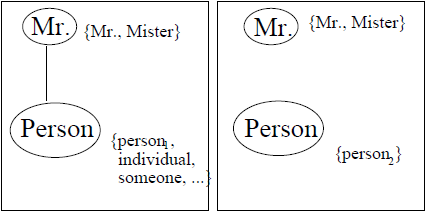
\includegraphics[keepaspectratio=true,width=0.9\columnwidth]{step_1_int_1_2.PNG}
    \caption{��� 1, ������������� 1 (�����) � 2 (������)}
    \label{step1}
\end{figure*}

\begin{figure*}
        \centering
        \begin{subfigure}[b]{0.33\textwidth}
                \fbox{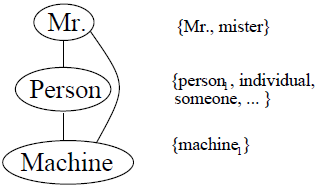
\includegraphics[width=\textwidth]{step_2_int_1.PNG}}
%                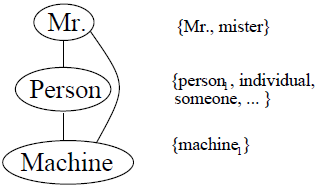
\includegraphics[width=\textwidth]{step_2_int_1.PNG}
%                \caption{��� 2, ������������� 1}
                \caption{������������� 1}
        \end{subfigure}%
%        \hfill%%% horizontal distance between two images (side by side)
        \quad% add desired spacing between images, e. g. ~, \quad, \qquad, \hfill etc.
             % (or a blank line to force the subfigure onto a new line)
        \begin{subfigure}[b]{0.39\textwidth}
                \fbox{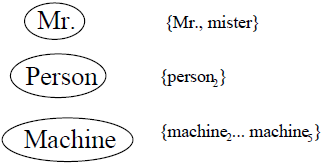
\includegraphics[width=\textwidth]{step_2_int_2.PNG}}
%                \caption{��� 2, ������������� 2}
                \caption{������������� 2}
        \end{subfigure}

        %~ %add desired spacing between images, e. g. ~, \quad, \qquad, \hfill etc.
          %(or a blank line to force the subfigure onto a new line)
        \begin{subfigure}[b]{0.39\textwidth}
                \fbox{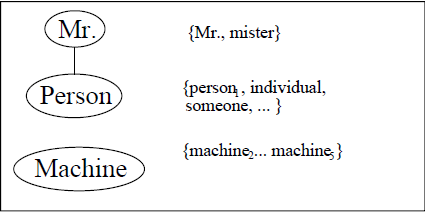
\includegraphics[width=\textwidth]{step_2_int_3.PNG}}
%                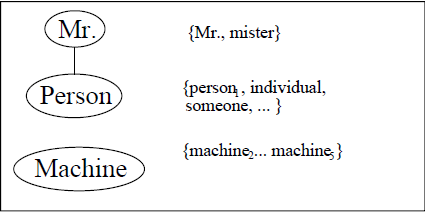
\includegraphics[width=\textwidth]{step_2_int_3.PNG}
%                \caption{��� 2, ������������� 3}
                \caption{������������� 3}
        \end{subfigure}
%        \hfill%%% horizontal distance between two images (side by side)
        \quad% add desired spacing between images, e. g. ~, \quad, \qquad, \hfill etc.
             % (or a blank line to force the subfigure onto a new line)
        \begin{subfigure}[b]{0.33\textwidth}
                \fbox{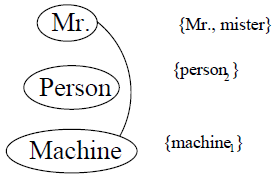
\includegraphics[width=\textwidth]{step_2_int_4.PNG}}
%                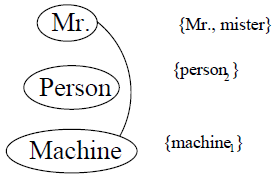
\includegraphics[width=\textwidth]{step_2_int_4.PNG}
%                \caption{��� 2, ������������� 4}
                \caption{������������� 4}
        \end{subfigure}
        \caption{������ ������������� �� ������ ����}\label{step2}
\end{figure*}

\begin{figure*}
        \centering
        \begin{subfigure}[b]{0.42\textwidth}
                \fbox{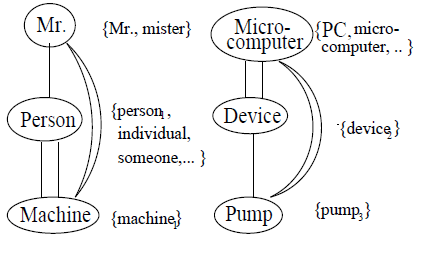
\includegraphics[width=\textwidth]{step_3_int_1.PNG}}
%                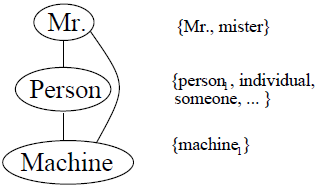
\includegraphics[width=\textwidth]{step_2_int_1.PNG}
%                \caption{��� 2, ������������� 1}
                \caption{������������� 1}
        \end{subfigure}%
        \quad% add desired spacing between images, e. g. ~, \quad, \qquad, \hfill etc.
             % (or a blank line to force the subfigure onto a new line)
        \begin{subfigure}[b]{0.42\textwidth}
                \fbox{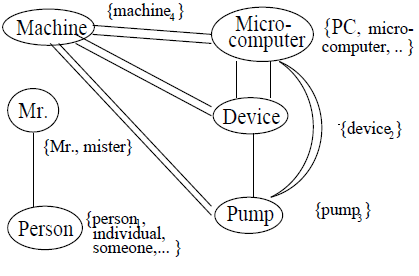
\includegraphics[width=\textwidth]{step_3_int_2.PNG}}
%                \caption{��� 2, ������������� 2}
                \caption{������������� 2}
        \end{subfigure}
        \caption{��� ����� ������� �������������, ���������� �� ������� ����}\label{step6}
\end{figure*}

������ ������������� ������������ ��� ����� ������ �� �������. 
������ ������� ������������ ����������� � ����� ��������� ����� ����������� �������. 
� ������������ ������ ������������� ��������� ���: ���������� � ��������~-- 10, ��������~-- 7, 
���������� � ��������~-- 4. ��������� �������� ��������� ��� ��������� �������������, 
�� �������� ������������ ����� ����. 
����� ����� ��������� ������������� ��������� ������������ �����, ������ ������������� ���������, 
��� ���������� ��� �������������� ����������������� ����� ��������\-����� ������.

\textbf{����������� ������� �� ������ ���������.} ����� �������������� ����������� �� �������� (��������� ����������� ��� �����). ������ ���� (\textit{Mr. Kenny...}) ������������� ������ ��������. ������� �������� ��� ������� �������� �� ������ ��������� ��������� ����� ������� (extra-strong, strong, medium-strong). �� ��������� ����� ������������ ������� �� ������ ���������, �� ��� ����������� �����, ����� ����������� ��� ����� ������� �������: ��� ������� ������������, ���� ��� �������� ���� � �� �� ����� � ����� � ��� �� ��������. ��������� ���� ������ ����� ����� ��������� � ���������� ������� ������, ��������� � ������� ����������� ������� ����� ������ � �������� ������~-- ��������� ������ �� ��������~\cite{Barzilay Elhadad 1997}.

\textbf{���������� ������ �������.} ��� ���� ����� ������������ ����������� ������� ��� ���������� ���������, � ������ ������� ������� ������� ���������� ������� ����� ���� ���, ������� ��������� ��������� ���� ����������. �������� � �������� �~\cite{Barzilay Elhadad 1997}  ����������  ������������ �������� ��� ������ ���� �������. ��� ����������� �����, ����� ��������� � ���������� ��������������� ����������� �������, ����� ������� ����������������, ��������� ������ ���������������� (������������) �������� ���� �������. ������ ������� ������ �� 30 �������, ��������� ��������� ������� �� ���������� �������� (��������, <<The Economist>>, <<Scientific American>>). ��� ������� ������ ������� ��������� ������������ ������� �� ������� ������������ �������� ����� ������. 

�� ��������� ����������, ������� ����� �������� (����� �������; ����� ������, ������������ ��������; ���������; ������� ���� ������� � ����� ���������; ����� ����������), �������� � �������� \cite{Barzilay Elhadad 1997} ������� ����� ����� ��������� ���������� ���������� ������� ��� ���������� ��������:

\begin{itemize}
\item \textit{����� (Length):} ����� ������������ � ������ ��������� �������.
\item \textit{������ ������������ (HomogeneityIndex):} 1~-- ���������� ��������� ������������ � ������ ��������� �������, �������� �� ����� (\textit{Length}).
\end{itemize}

����� �������, ���������� ������� ����������� ���:
\begin{equation*}
\text{Score(Chain)} = \text{Length} \times \text{HomogeneityIndex}
\end{equation*}

��� ������������ ������� � ������������ � ���� ������� ���� �������, ��� ��� ���������� �������� ����� �������, ��������������� <<�������� ��������� (����)>>:
\begin{equation*}
\begin{split}
\text{Score(Chain)} > \text{Average(Scores)} + \\
2 \times \text{StandardDeviation(Scores)},
\end{split}
\end{equation*}

\noindent��� \textit{Average}~-- ��� ������� ������ �� ���� ��������, \textit{StandardDeviation}~-- �������������������� ����������.

\textbf{���������� ������ �����������.} ����� ���� ��� ������� ������� ��������, ����������� ����� ��������������� �� ����������� � ���������� ���� ����������� ������� �� ��������� ������.

��� ������ ������� ������� �� ������ ������������� �������� ���������� ����� ���� ����������� ��� ��������� � ����� ��������:

\underline{��������� 1:} ��� ������ ������� ��� ��������� � ������� ������� �� �����������, ������� �������� ������ ��������� ����� ������� � ������.

\underline{��������� 2:} ��� ������ ������� ��� ��������� � ������� ������� �����������, ������� �������� ������ ��������� \textit{��������������} �������� ������� � ������. \textit{�������������} ����� (representative words), �������� ��������������� �������,~-- ��� ����� ����� �������, ������� ����������� � ������� �� ����, ��� � ������� �� ���� ������ �������.

\underline{��������� 3:} ��� ������ ���� ����� ���� ������, ��� ���� ������� ������������ ������� (�. �. ����� ������������ ��������� �� ���� �������). ������� ����������� � ������� ��������� ������� � ���� �����. ������������ ����������� ��� ����� ��������� ������ ���� � ��������, ����������� �� ���������� ��������������� � ��������. ������� ����� ������� ������������, ���� �� ������������ �������� ������������ �� ���� �������. ������� ������������ ����� ������ ���������������� ���������, �����, ��� ������ ������� �������� �����-���� �������� �������.

������������ � \cite{Barzilay Elhadad 1997} �������� ������������ ������������ ��������� �� ������ ����������� ������� (�������� 47--61\,\% � ������� 64--67\,\%) �� ��������� � ���������� Microsoft Summarizer, ��������� � Word�97 (�������� 32--33\,\% � ������� 37--39\,\%). ��� ���������� ��������� �� ������� ��������� ����������� ������� � ������ �������������.


\section{���������� �������������� ����������� �� ������ ����������� \mbox{�����} ��� ���������� ��������������}
\begin{flushright}
\textit{�. �. ��������} 
\end{flushright}

� ������ \cite{Ciaramita 2000} ������������ ����������� ������, ����������� ��� ���������� ����������� �������������� ��������. ������ ������������� ����� �������, ��� �������������� ����������� (selectional preferences). \textit{�������������� �����������} (����� SP) --- ��� �������������� ������������� ������� ������������ �������������� ������ ��� ���������� (�������, ������ (������ ����������) � ��������� ����������).

������ ��������������� ���������� SP ����� ���� �� ���� � ����� ���������� � ��������� ������������� �����. �������������� ����������� ������� ����� ����������� ��� ��������� ��������� �������� ������������ ��������� ��� ��������� ��������; ��������, �� ����������� \textit{<<������� ���� ������� � ������ �� ������>>} ����� ����������, ��� �xxxx� --- ����. ��� ���������� ����������� SP ��������� ������������� �������� � ������� ������ ����� ���. ������������ SP ����� �� ������ � ��������� ��������� ����������� ���������. 

������� �������� SP ��� ������� ������ ����������� �������������� ������� � �������, ���������� �� �������. ��������� ���� ������ (����� WordNet \cite{Miller 1990}) --- ��� ������ ���� ������, � ������� ����� ������������� � ������. 

�������������� ��������� ������� �� ��� ��������-��������, ����������� �� �������������� �������. � ����������� ��������� ����� ���� �� �������� ������ ���� (������ ���������� �������), � ��� ��� ����, ������� ���� � WordNet, ������� �� ������������� ������. � ������ \cite{Ciaramita 2000} ������������� ������� ���������� \textit{������}  ��������� WordNet, �. �. ����� ������������� ������ �� �������� �����. ����� �������, � ����������� ��������� �� ������ ������ WordNet ����� ������� ������ (�������� ����), � �������� ������������� (����������� � �������) �������.

��������, ���� � �������� ������� ������� ������ \textit{�������} ������������� �� ������ \textit{�������}, ������������� ������ ��������, �� � ������ ���������� SP ����� ��������, ��� <<������ \textit{�������} ������������� �� ������� �� ������ ��������>>. ���� ����� \textit{��������}, ��-������, ����� ����������� � ������ � �������� \textit{�������}, ��-������, ����� \textit{��������} ����������� ����� ���� �������: �������� � ��������, �� �� ����� �������, ��� ������ SP ����� ��������� ����������� � ���, ��� ������� \textit{�������} ������������� �� ������� �� ������� � ��������, � �������һ.

� ����� ������������� ������� (������ (1997) \cite{Resnik 1997}, ���� � ���� (1999) \cite{Abney 1999}) ���� ����������, ��� ������� ��������� � ����� ����������� ��������� --- ��� ������� ������������� ���� � ��������� ������. � ��� �� ������� (\cite{Resnik 1997}, \cite{Abney 1999}) ���� ���������� ����� ������� ������, � ������� ��������������, ��� ��� �������� ������������ ���� ���������� � ���������� ��������. 

\textbf{����������� ����}, ��� ����������� \mbox{����} ������� (���), ������� �� ��������� ����\-������ (������) � ��������� ��������������� �����, ����������� ��� ����������. ����� ���� ������������� ��������������� ������������ ����. ������ ���������� ����� ��������� ���� �� ��������� ����� ����������������� ���������. ����� ��� ���������� ����� ��������� ����, �. �. ��������� ���� �� ���� ��������: ������ ��� ����. ����� ���������� \textit{�} � ���������� $B_1,... , B_n$ ������������� ������� �������� ������������ (conditional probability table, ����� CPT).

��������, �������� SP ��� ������� \textit{�������}, � ���� �� ���.~\ref{ris1} ����� ����� ������.
\begin{figure}[H]
    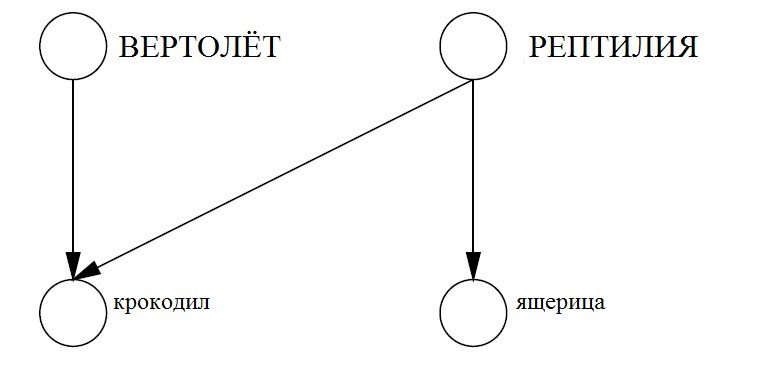
\includegraphics[keepaspectratio=true,width=0.9\columnwidth]{bayesian_network_crocodile.jpg}
    \caption{����������� ���� ��� ������������� ���������������� \textit{��������}}
    \label{ris1}
\end{figure}

������ \textit{�������} ������������� �� ������� \textit{��������} � \textit{�������}. ���������� �������� � �������� ������������� ����� ����� ����������� ���������, ���������� \textit{��������} � \textit{�������} �������� ����� ������, ����������� ����������. ���������� �������� ����� ��������� ���� �� ���� ��������, ��������������� ������ \textit{��������} � \textit{�������}, ������ ��� ������ ����������� �������� � ����� ������.

\begin{table}[H]
\centering
\caption{�������� ����������� ���������� \textit{��������} � \textit{�������} � ����������� �� �������� ���������� �������� � ��������, ��� (�, �, �, � --- ��� ������������ ���� ��������, ��������, \textit{��������} � \textit{�������})}
\begin{tabular}{|c|c|c|c|c|}
\hline
 & \multicolumn{4}{c|}{ } \\
" " & \multicolumn{4}{c|}{ $P(X=x|Y_1=y_1,Y_2=y_2)$ } \\
 & \multicolumn{4}{c|}{ } \\
\hline
 & &  &  & \\
" " & �, � & �, \textlnot � & \textlnot �, � & \textlnot �, \textlnot �\\
  & &  &  & \\
\hline
  & &  &  & \\
� = \textit{true} & 0,99 & 0,99 & 0,99 & 0,01\\
� = \textit{false} & 0,01 & 0,01 & 0,01 & 0,99\\
 & &  &  & \\
\hline
  & &  &  & \\
� = \textit{true} & 0,99 & 0,99 & 0,01 & 0,01\\
� = \textit{false} & 0,01 & 0,01 & 0,99 & 0,99\\
 & &  &  & \\
\hline
\end{tabular}
\label{tbl1}
\end{table}

��� ���������� ����.~\ref{tbl1} �������� ������������ (CPT) ����� ��������� �������������:
\begin{itemize}
\item �����������, ��� �������� �����-���� �� ��������� (�������� � ��������) ����� ����, �. �. \textit{P}(\textit{�\,=\,true}) = \textit{P}(\textit{�\,=\,true}) = 0,01, �������������, ������ �����������, ��� �������� �� �������: \textit{P}(\textit{�\,=\,false}) = \textit{P}(\textit{�\,=\,false}) = 0,99;
\item ���� �����-���� �� ��������� ������� (�, �), �� <<��������>> ����� \textit{��������};
\item ���� ������� �������� �������, �� ������ ����� ��������� ����� \textit{�������}.
\end{itemize}

�� ����.~\ref{tbl1} ����������� ��������� ���� ������� �����, ��� ������������� ����� ���� �������� ����� \textit{�������� (�������� � �������� ��-24)} ������������. ����������� ������������� �������� �������� ������� ������, ��� �������� ��������. ����� �������, �������� <<��������>> <<���������>> (<<explaining away>>).

\textbf{����������� ���� ��� ���������� SP.} 
�������� ��������������� � WordNet ������������ � ���� ���������������� ������������� �����. 
������ ���� ��������� �������� <<������>>, ���� ������ <<��������>> ��������������� �� ������ ���������. 
��������� ����������� �������� �� ������ ���� �������������: ��-������, ������������, 
��� ������ ����� ������������� ������ �� ������� ������-�� ����������� �������, 
� ��-������, ���� ������ ������������� ������������� ������ �� ������� �� ������� ������� (��������, ������ ���), 
����� ������ ���� ����������� ������������ ����� ������� � ���������� ����� ������� (��������, �����).

�� �� ������������� (��� ��� ��������) ����� � ��� ������������ ���� � ���������:
\begin{enumerate}
\item �����, ��������, �������� ���������� ������� � ��� ������, ���� ������ ������������� � �����-���� �� �������� ����� �����;
\item ���������� ������ ������-������ ������� � ����� ����������� ����, ��� ����� ����� ������� ������������� � ��������.
\end{enumerate}

������ <<��������>> � <<������������>> ������ ���� ��������� ����� �����, ����� ������� ����� �������. 

�������� ������ \cite{Ciaramita 2000} �������� ����������� ��������� <<explaining away>>, �. �. ������������ ������������� �������� ���� ��� ���������� �������������� �����������. ����� ��������� �������� ������������ ��������� ����������� ����� � ������������ ������, �������� ��������� ��� ���������� ����������� ��������������. 

\section{Заключение}

Разрешение лексической многозначности - это задача выбора между разными значениями слов и словосочетаний в словаре в зависимости от контекста. Задача разрешения лексической многозначности является открытой проблемой, то есть крайне интересной и привлекательной с научной точки зрения.

В статье представлен краткий обзор методов и алгоритмов разрешения лексической многозначности. Во-первых, методы, основанные на машинном обучении.  Во-вторых, методы, не использующие никаких размеченных корпусов для различения значений слов. В-третьих, методы, использующие внешние словарные источники информации (машиночитаемые словари, тезаурусы, онтологии).

Работа Старковой В.Г. поддержана грантом РГНФ (проект № 15-04-12029), работа Кириллова А.Н. и Чирковой Ю.В. поддержана грантом РГНФ (проект № 15-04-12006). Работа Крижановского А. А. выполнена при частичной финансовой поддержке Программы фундаментальных исследований Секции литературы и языка ОИФН РАН «Язык  и информационные технологии» 2015-2017 (проект «Корпус вепсского языка: разработка и формирование морфологической базы электронного ресурса»).
 
\begin{thebibliography}{9}

\bibitem{Averin 2006}
\textit{Аверин А. Н.} Разработка сервиса поиска биграмм // Труды международной конференции «Корпусная лингвистика–2006. СПб., С.Петерб. ун-та., 2006. С. 5~ - 15.

\bibitem{epr:website}
\textit{Епрев А. С.} Применение контекстных векторов в классификации текстовых документов // 
“Журнал радиоэлектроники”.   2010. N 10. URL: http://jre.cplire.ru/iso/oct10/1/text.html (дата обращения: ).

\bibitem{Kim 1989}
\textit{Ким Дж. О., Мьюллер Ч. У., Клекка У. Р.} Факторный, дискриминантный и кластерный анализ / <<Финансы и статистика>>, Москва, Россия. 1989. Стр.172.

\bibitem{Lukash 2011}
\textit{Лукашевич Н. В.} Тезаурусы в задачах информационного поиска / Издательство МГУ, 2011. 495 с.

\bibitem{Trudakov 2010}
\textit{Турдаков Д. Ю.} Методы и программные средства разрешения лексической многозначности терминов на основе сетей документов: дис. … канд. физико-математических наук:  Москва, 2010.  138 c.

\bibitem{Abney 1999}
\textit{Abney S. and Light M.} Hiding a semantic hierarchy in a markov model. In Proceedings of the Workshop on Unsupervised Learning in Natural Language Processing, ACL. 1999.

\bibitem{Azzini}
\textit{Azzini A., da Costa Pereira C., Dragoni M. and Tettamanzi A. G. B.} Evolving Neural Networks for Word Sense Disambiguation // 8-th International conference on hybrid intelligent systems. Spain. Barcelona, 2008. P. 332–337. doi: 10.1109/HIS.2008.88

\bibitem{Barzilay Elhadad 1997}
\textit{Barzilay R. and  Elhadad M. }Using lexical chains for text summarization // In Proceedings of the ACL Workshop on Intelligent Scalable Text Summarization (Madrid, Spain). 1997. P. 10–17.

\bibitem{Berry 1993}
\textit{Berry M.,  Do T.,  O’Brien G.,  Krishna V. and Varadhan S. }SVDPACK (version 1.0) user’s guide. Technical Report CS-93-194, University of Tennessee at Knoxville, Computer Science Department, April 1993.

\bibitem{Bruce 1994}
\textit{Bruce R. and  Wiebe J. }Word-sense disambiguation using decomposable models // In Proceedings of the 32nd Annual Meeting of the Association for Computational Linguistics, 1994. P. 139–146. doi: 10.3115/981732.981752

\bibitem{Wu}
\textit{Carpuat M. and Wu D.}Evaluating the Word Sense Disambiguation Performance of Statistical Machine Translation. URL: http://www.aclweb.org/anthology/I05-2021 (дата обращения: 14.05.2015)

\bibitem{Ciaramita 2000}
\textit{Ciaramita M. and  Johnson M. }Explaining away ambiguity: Learning verb selectional preference with Bayesian networks. 2000. 

\bibitem{COTTRELL 1983}
\textit{Cottrell G. W. and  Small S. L. }A connectionist  scheme for modelling word  sense  disambiguation // Cognition and brain theory. 1983. № 6. P. 89–120. 

\bibitem{COTTRELL 1989}
\textit{Cottrell G. W. }A connectionist approach to word sense disambiguation / Pitman, London, 1989.

\bibitem{Do Thuy Duong 2011}
\textit{Duong D. T. }Automated text summarization. Graduation Thesis. Hanoi University. 2011. 

\bibitem{Donald 1990}
\textit{Hindle D. }Noun classification from predicate-argument structures // In Proceedings of ACL-90, Pittsburg, Pennsylvania, June, 1990. P. 268-275.

%\bibitem{Charles 1993}
%\textit{Ling Charles X.,  Marinov M. }Answering the connectionist challenge: A symbolic model of learning the past tenses of English verbs,  %Cognition, Elsevier, 1993.

%\bibitem{Dekang 1998}
%\textit{Lin D. }Automatic Retrieval and Clustering of Similar Words.Proceedings of the 17th international conference on Computational %linguistics-Volume 2. – Association for Computational Linguistics, Department of Computer Science University of Manitoba Winnipeg, Manitoba, %Canada, 1998, pp. 768-774. DOI: 10.3115/980432.980696

%\bibitem{Dekang 1993}
%\textit{Lin D. }Principle-based parsing without overgeneration. In Proceedings of ACL-93, Columbus, Ohio, 1993, pp. 112-120. DOI: %10.3115/981574.981590

%\bibitem{Dekang 1997}
%\textit{Lin D. }Using syntactic dependency as local context to resolve word sense ambiguity. In Proceedings of ACL/EACL-97, Madrid, Spain, %July, 1997, pp. 64-71. DOI: 10.3115/979617.979626

%\bibitem{Donald 1990}
%\textit{Hindle D. }Noun classification from predicate-argument structures. In Proceedings of ACL-90, Pittsburg, Pennsylvania, June, 1990, pp. %268-275.

%\bibitem{Do Thuy Duong 2011}
%\textit{Duong D. T. }Automated text summarization. Graduation Thesis. Hanoi University. 2011. 

\bibitem{Freund 1999}
\textit{Freund Y., Schapire R. E. }A Short Introduction to Boosting // AT\&T Labs Research, Shannon Laboratory.  1999.

\bibitem{Freund 1996}
\textit{Freund Y.,  Schapire R. E. }Game theory, on-line prediction and boosting // In Proceedings of the Ninth Annual Conference on Computational Learning Theory,  1996. P. 325-332.

\bibitem{Freund 1997}
\textit{Freund Y.,  Schapire R. E. }A decision-theoretic generalization of on-line learning and an application to boosting // Journal of Computer and System Sciences. 1997. P. 119–139. doi: 10.1006/jcss.1997.1504

\bibitem{Halliday Hasan 1976}
\textit{Halliday M. and  Hasan R. }Cohesion in English / London: Longman. 1976. 

\bibitem{Harris 1985}
\textit{Harris Z. }Distributional structure / In: Katz, J. J. (ed.) The Philosophy of Linguistics. New York: Oxford University Press. 1985. P. 26–47

\bibitem{Hearst 1994}
\textit{Hearst M. }Multi-paragraph segmentation of expository text // In Proceedings of the 32th Annual Meeting of the Association for Computational Linguistics, 9–16. Las Cruces, New Mexico: Association for Computational Linguistics. 1994. doi: 10.3115/981732.981734

\bibitem{Hinton 1986}
\textit{Hinton G. E.,  McClelland J. L.,  Rumelhart D. E.. }Distributed representations // In Parallel Processing: explorations in the microstructure of cognition. MIT Press, Cambridge, MA, 1986. P. 5–44.

\bibitem{Hirst St-Onge 1998}
\textit{Hirst G. and  St-Onge D. }Lexical chains as representations of context for the detection and correction of malapropisms. WordNet: An electronic lexical database, 1998. P. 305-332.

\bibitem{Hoey 1991}
\textit{Hoey M. }Patterns of Lexis in Text / Oxford: Oxford University Press. 1991. 

\bibitem{Jain 1988}
\textit{Jain A. and  Dubes R. }Algorithms for Clustering Data / Prentice-Hall, Inc., Upper Saddle River, NJ, 1988.

\bibitem{Jain 1999}
\textit{Jain A.,  Murthy M. and  Flynn P. }Data clustering: a review // ACM Computing Surveys, 31(3):264-323, September 1999. doi: 10.1145/331499.331504

\bibitem{Leacock 1993}
\textit{Leacock C.,  Towell G. and  VoorheesE. }Corpus-based statistical sense resolution // In Proceedings of the ARPA Workshop on Human Language Technology, March. 1993, P. 260–265.  

\bibitem{LESK 1986}
\textit{Lesk M. }Automatic sense disambiguation using machine readable dictionaries: How to tell a pine cone from an ice cream cone //  Proceedings  of  the 5th SIGDOC. New York. 1986. P. 24–26. doi: 10.1145/318723.318728

\bibitem{Dekang 1998}
\textit{Lin D. }Automatic Retrieval and Clustering of Similar Words // Proceedings of the 17th international conference on Computational linguistics-Vol. 2. –  Department of Computer Science University of Manitoba Winnipeg, Manitoba, Canada, 1998, P. 768-774. doi: 10.3115/980432.980696

\bibitem{Dekang 1993}
\textit{Lin D. }Principle-based parsing without overgeneration // In Proceedings of ACL-93, Columbus, Ohio, 1993, P. 112-120. doi: 10.3115/981574.981590

\bibitem{Dekang 1997}
\textit{Lin D. }Using syntactic dependency as local context to resolve word sense ambiguity // In Proceedings of ACL/EACL-97, Madrid, Spain, July, 1997, P. 64-71. doi: 10.3115/979617.979626


\bibitem{Lin 2001}
\textit{Lin D. and Pantel P. }Induction of semantic classes from natural language text // In Proceedings of SIGKDD-01. San Francisco, CA. 2001. P. 317–322. doi: 10.1145/502512.502558  

\bibitem{Charles 1993}
\textit{Ling Charles X.,  Marinov M. }Answering the connectionist challenge: A symbolic model of learning the past tenses of English verbs /  Cognition, Elsevier, 1993.


\bibitem{Manning 1999}
\textit{Manning C. D. and  Sch\"utze H. }Foundations of Statistical Natural Language Processing / MIT Press. 1999.

\bibitem{Merz 1998}
\textit{Merz C. J. and  Murphy P. M. }UCI repository of machine learning databases, 1998. URL: www.ics.uci.edu/ mlearn/MLRepository.html (дата обращения: 24.04.2015).

\bibitem{Miller 1990}
\textit{Miller G. }Wordnet: An on-line lexical database // International Journal of Lexicography, 3(4). 1990.

\bibitem{Mooney 1996}
\textit{Mooney R. J. }Comparative Experiments on Disambiguating Word Senses:
An Illustration of the Role of Bias in Machine Learning / Department of Computer Sceinces, University of Texas, Austin, TX 78712-1188, 1996.

\bibitem{Mooney 1995}
\textit{Mooney R. J., Califf M. E. }Induction of First-Order Decision Lists: Results on Learning the Past Tense of English Verbs / Department of Computer Sceinces, University of Texas, Austin, TX 78712-1188, 1995.

\bibitem{Morris Hirst 1991}
\textit{Morris J. and  Hirst G. }Lexical cohesion computed by thesaural relations as an indicator of the structure of text // Computational Linguistics 17(1):21–43. 1991. 

\bibitem{Navigli 2009}
\textit{Navigli R. }Word sense disambiguation: A survey. ACM Computing Surveys (CSUR) 41, no. 2 (2009): 10. doi: 10.1145/1459352.1459355

\bibitem{Eugene 1975}
\textit{Nida Eugene A. }Componential Analysis of Meaning / The Hague, Mouton. 1975.


\bibitem{Pantel 2002}
\textit{Pantel P.,  Lin D. }Discovering Word Senses from Text / University of Alberta. Department of Computing Science Edmonton, Alberta T6H 2E1 Canada, 2002. doi: 10.1145/775047.775138

\bibitem{Pedersen 2000}
\textit{Pedersen T. }A Simple Approach to Building Ensembles of Naive Bayesian Classifers for Word Sense Disambiguation / Department of Computer Science, University of Minnesota Duluth. 2000.

\bibitem{Pedersen 1997}
\textit{Pedersen T. and  Bruce R. }Distinguishing word senses in untagged text / Proc.EMNLP.Providence, RI, 1997.

\bibitem{Purandare 2004}
\textit{ Purandare A. and  Pedersen T. }Improving word sense discrimination with gloss augmented feature vectors // Workshop on Lexical Resources for the Web and Word Sense Disambiguation.  2004.  P. 123-130. 

\bibitem{Quinlan 1993}
\textit{Quinlan J. R. }C4.5: Programs for Machine Learning / Morgan Kaufmann, 1993. 

\bibitem{Resnik 1997}
\textit{Resnik P. }Selectional preference and sense disambiguation / In Proceedings of the ANLP-97 Workshop: Tagging Text with Lexical Semantics: Why, What, and How? 1997.

\bibitem{Savova 2005}
\textit{Savova G., Pedersen T., Purandare A., Kulkarni A. }Resolving ambiguities in biomedical text with unsupervised clustering approaches / University of Minnesota Supercomputing Institute Research Report, 2005.
                          
\bibitem{Schapire 1998}
\textit{Schapire R. E. and Singer Y. }Improved boosting a predictions // In Proceedings of the Eleventh Annual Confere Theory, 1998. P. 80–91. 

\bibitem{Schapire 1997}
\textit{Schapire R. E. }Using output codes to boost multiclass learning problems. In Machine Learning // Proceedings of the Fourteenth International Conference, 1997. P. 313–321. 

\bibitem{Schutze 1998}
\textit{Sch$\ddot{u}$tze H. }Automatic Word Sense Discrimination // Computational Linguistics, vol. 24, number 1., 1998.

\bibitem{SC:website}
\textit{SenseClusters. }  \newline URL: http://senseclusters.sourceforge.net (дата обращения: 24.04.2015).

\bibitem{UMLS:website}
\textit{UMLS Terminology Services (UTS).} URL: http://umlsks.nlm.nih.gov/kss/servlet/Turbine/\newline template (дата обращения: 22.04.2015)

\bibitem{VERONIS 1990}
\textit{Veronis J. and Ide N. }Word  sense  disambiguation  with  very  large neural  networks  extracted  from machine readable dictionaries // Proceedings of the 13th International Conference on Computational Linguistics. Helsinki. 1990. P. 389–394. doi: 10.3115/997939.998006

\bibitem{WALTZ 1985}
\textit{Waltz D. L. and  Pollack J. B. }Massively parallel parsing: a strongly interactive  model  of  natural  language interpretation // Cognitive science. 1985. № 9. P. 51–74. doi: 10.1207/s15516709cog0901\_4
                     
\bibitem{Weeber 2001}
\textit{Weeber M.,  Mork J.,  Aronson A. }Developing a test collection for biomedical word sense disambiguation / Proc. AMIA., 2001.

\bibitem{Zhao 2002}
\textit{Zhao Y. and  Karypis G. }Evaluation of hierarchical clustering algorithms for document datasets // In Proceedings of the 11th International Conference on Information and Knowledge Management, McLean, VA, 2002. P. 515-524. doi: 10.1145/584792.584877



\end{thebibliography}
\end{articletext}


\section{СВЕДЕНИЯ ОБ АВТОРE:}

\begin{aboutauthors}
\authorsname{Каушинис Татьяна Викторовна}
Студентка\\
Математический факультет\\ 
Петрозаводский государственный университет\\
пр-кт Ленина, 33, Петрозаводск, Республика Карелия\\
тел.: (8142) 711078\\
эл. почта: merilstreet@mail.ru

\columnbreak

\authorsname{Kaushinis, Tatiana}
Petrozavodsk State University\\
33, Lenin Str., 185910, Petrozavodsk, Republic of Karelia, Russia\\
tel.: (8142) 711078\\
e-mail: merilstreet@mail.ru
\end{aboutauthors}

\begin{aboutauthors}
\authorsname{Кириллов Александр Николаевич}
Доктор физико-математических наук\\ 
доцент\\
Институт прикладных математических исследований Карельского научного центра РАН\\ 
ул. Пушкинская, 11, Петрозаводск, Республика Карелия, Россия, 185910\\
эл. почта: kirillov@krc.karelia.ru\\
тел.: (8142) 766312

\columnbreak

\authorsname{Kirillov, Alexander}
Institute of Applied Mathematical Research, Karelian Research Centre, Russian Academy of Sciences\\
11, Pushkinskaya St., 185910 Petrozavodsk, Karelia, Russia\\
e-mail: kirillov@krc.karelia.ru\\
tel.: (8142) 766312
\end{aboutauthors}

\begin{aboutauthors}
\authorsname{Коржицкий Никита Иванович}
Студент\\
Математический факультет\\ 
Петрозаводский государственный университет\\
пр-кт Ленина, 33, Петрозаводск, Республика Карелия\\
тел.: (8142) 711078\\
эл. почта: nikita@nikita.tv

\columnbreak

\authorsname{Korzhitsky, Nikita}
Petrozavodsk State University\\
33, Lenin Str., 185910, Petrozavodsk, Republic of Karelia, Russia\\
tel.: (8142) 711078\\
e-mail: nikita@nikita.tv 
\end{aboutauthors}

\begin{aboutauthors}
\authorsname{Крижановский Андрей Анатольевич}
Кандитат технических наук\\ 
Институт прикладных математических исследований Карельского научного центра РАН\\ 
ул. Пушкинская, 11, Петрозаводск, Республика Карелия, Россия, 185910\\
эл. почта: andew.krizhanovsky@gmail.com\\
тел.: (8142) 766312

\columnbreak

\authorsname{Krizhanovsky, Andrew}
Institute of Applied Mathematical Research, Karelian Research Centre, Russian Academy of Sciences\\
11, Pushkinskaya St., 185910 Petrozavodsk, Karelia, Russia\\
e-mail: andew.krizhanovsky@gmail.com\\
tel.: (8142) 766312
\end{aboutauthors}

\begin{aboutauthors}
\authorsname{Пилинович Александр Владимирович}
Студент\\
Математический факультет\\ 
Петрозаводский государственный университет\\
пр-кт Ленина, 33, Петрозаводск, Республика Карелия\\
тел.: (8142) 711078\\
эл. почта: alexander.pilinovich@yandex.ru

\columnbreak

\authorsname{Pilinovich, Aleksander}
Petrozavodsk State University\\
33, Lenin Str., 185910, Petrozavodsk, Republic of Karelia, Russia\\
tel.: (8142) 711078\\
e-mail: alexander.pilinovich@yandex.ru 
\end{aboutauthors}

\begin{aboutauthors}
\authorsname{Сихонина Ирина Александровна}
Студентка\\
Математический факультет\\ 
Петрозаводский государственный университет\\
пр-кт Ленина, 33, Петрозаводск, Республика Карелия\\
тел.: (8142) 711078\\
эл. почта: syawenka@mail.ru

\columnbreak

\authorsname{Sikhonina, Irina}
Petrozavodsk State University\\
33, Lenin Str., 185910, Petrozavodsk, Republic of Karelia, Russia\\
tel.: (8142) 711078\\
e-mail: syawenka@mail.ru 
\end{aboutauthors}

\begin{aboutauthors}
\authorsname{Спиркова Анна Михайловна}
Студентка\\
Математический факультет\\ 
Петрозаводский государственный университет\\
пр-кт Ленина, 33, Петрозаводск, Республика Карелия\\
тел.: (8142) 711078\\
эл. почта: annspirkova@gmail.com

\columnbreak

\authorsname{Spirkova, Anna}
Petrozavodsk State University\\
33, Lenin Str., 185910, Petrozavodsk, Republic of Karelia, Russia\\
tel.: (8142) 711078\\
e-mail: annspirkova@gmail.com
\end{aboutauthors}

\begin{aboutauthors}
\authorsname{Старкова Валентина Геннадьевна}
Старший инженер-программист\\ 
Институт прикладных математических исследований КарНЦ РАН\\ 
ул. Пушкинская, 11, Петрозаводск, Республика Карелия, Россия, 185910\\
тел.: (8142) 766312\\
эл. почта: stark\_val@mail.ru

\columnbreak

\authorsname{Starkova, Valentina}
Institute of Applied Mathematical Research, Karelian Research Centre, Russian Academy of Sciences\\
11, Pushkinskaya St., 185910 Petrozavodsk, Karelia, Russia\\
tel.: (8142) 766312\\
e-mail: stark\_val@mail.ru 
\end{aboutauthors}

\begin{aboutauthors}
\authorsname{Степкина Татьяна Владимировна}
Студентка\\
Математический факультет\\ 
Петрозаводский государственный университет\\
пр-кт Ленина, 33, Петрозаводск, Республика Карелия\\
тел.: (8142) 711078\\
эл. почта: hogdp@mail.ru

\columnbreak

\authorsname{Stepkina, Tatiana}
Petrozavodsk State University\\
33, Lenin Str., 185910, Petrozavodsk, Republic of Karelia, Russia\\
tel.: (8142) 711078\\
e-mail: hogdp@mail.ru
\end{aboutauthors}

\begin{aboutauthors}
\authorsname{Ткач Станислав Сергеевич}
Студент\\
Математический факультет\\ 
Петрозаводский государственный университет\\
пр-кт Ленина, 33, Петрозаводск, Республика Карелия\\
тел.: (8142) 711078\\
эл. почта: tkachkras@gmail.com

\columnbreak

\authorsname{Tkach, Stanislav}
Petrozavodsk State University\\
33, Lenin Str., 185910, Petrozavodsk, Republic of Karelia, Russia\\
tel.: (8142) 711078\\
e-mail: tkachkras@gmail.com 
\end{aboutauthors}

\begin{aboutauthors}
\authorsname{Чиркова Юлия Васильевна}
Кандидат физико-математических наук\\ 
Институт прикладных математических исследований КарНЦ РАН\\ 
ул. Пушкинская, 11, Петрозаводск, Республика Карелия, Россия, 185910\\
тел.: (8142) 766312
эл. почта: julia@krc.karelia.ru

\columnbreak

\authorsname{Chirkova, Julia}
Institute of Applied Mathematical Research, Karelian Research Centre, Russian Academy of Sciences\\
11 Pushkinskaya St., 185910 Petrozavodsk, Karelia, Russia\\
tel.: (8142) 766312
e-mail: julia@krc.karelia.ru
\end{aboutauthors}

\begin{aboutauthors}
\authorsname{Чухарев Алексей Леонидович}
Старший инженер-программист\\ 
Институт прикладных математических исследований КарНЦ РАН\\ 
ул. Пушкинская, 11, Петрозаводск, Республика Карелия, Россия, 185910\\
тел.: (8142) 766312
эл. почта: chuharev@krc.karelia.ru

\columnbreak

\authorsname{Chuharev, Alexey}
Institute of Applied Mathematical Research, Karelian Research Centre, Russian Academy of Sciences\\
11, Pushkinskaya St., 185910 Petrozavodsk, Karelia, Russia\\
tel.: (8142) 766312
e-mail: chuharev@krc.karelia.ru
\end{aboutauthors}

\begin{aboutauthors}
\authorsname{Шорец Дарья Сергеевна}
Студентка\\ 
Математический факультет\\ 
Петрозаводский государственный университет\\
пр-кт Ленина, 33, Петрозаводск, Республика Карелия\\
тел: (8142) 711078\\
эл. почта: da\_sha1078@mail.ru

\columnbreak

\authorsname{Shorets, Daria}
Petrozavodsk State University\\
33, Lenin Str., 185910, Petrozavodsk, Republic of Karelia, Russia\\
tel.: (8142) 711078\\
e-mail: da\_sha1078@mail.ru
\end{aboutauthors}

\begin{aboutauthors}
\authorsname{Ярышкина Екатерина Александровна}
Студентка\\ 
Математический факультет\\ 
Петрозаводский государственный университет\\
пр-кт Ленина, 33, Петрозаводск, Республика Карелия\\
тел:(8142) 711078\\
эл. почта: kate.rysh@gmail.com

\columnbreak

\authorsname{Yaryshkina, Ekaterina}
Petrozavodsk State University\\
33, Lenin Str., 185910, Petrozavodsk, Republic of Karelia, Russia\\
tel.: (8142) 711078\\
e-mail: kate.rysh@gmail.com 
\end{aboutauthors}

\begin{aboutauthors}
\authorsname{Янкевич Дарья Юрьевна}
Студентка\\ 
Математический факультет\\ 
Петрозаводский государственный университет\\
пр-кт Ленина, 33, Петрозаводск, Республика Карелия\\
тел: (8142) 711078\\
эл. почта: dyankevic@gmail.com

\columnbreak

\authorsname{Yankevich, Daria}
Petrozavodsk State University\\
33, Lenin Str., 185910, Petrozavodsk, Republic of Karelia, Russia\\
tel.: (8142) 711078\\
e-mail: dyankevic@gmail.com
\end{aboutauthors}


\end{document}
